% \pause
% \alert{text}
% \uncover<5->{\item foo}  al posto di \item
%\includegraphics[height=1cm]{moogle}
\documentclass{beamer}
\usepackage{graphicx}
%\usepackage{bcprules}
\usepackage{verbatim}
\usepackage{amsmath}
\usepackage{amssymb}
\usepackage{stmaryrd}
%\usepackage{stmaryrd}

% !TEX root = ../main.tex
%\usepackage{ulem}
%\input{\macrospath/ben-macros-diagrams.tex}
%\usepackage[usenames,dvipsnames,svgnames,table]{xcolor}

\newcommand{\sem}[1]{[\![#1]\!]}

%%%%%%%
%% LATEX SHORTCUTS
%%%%%%%
\newcommand{\ignore}[1]{}
\newcommand{\sep}{\hspace*{0.5cm}}
\newcommand{\ms}{\medskip}
\newcommand{\mathintitle}[2]{\texorpdfstring{#1}{#2}}
\newcommand{\colspace}{@{\hspace{.5cm}}}
\newcommand{\myinput}[1]{\ifthenelse{\boolean{withimages}}{\input{#1}}{}}
\newcommand{\spc}{@{\hspace{.5cm}}}

% for references
\newcommand{\reflemma}[1]{Lemma~\ref{l:#1}}
\newcommand{\reflemmap}[2]{Lemma~\ref{l:#1}.\ref{p:#1-#2}}
\newcommand{\reflemmaeq}[1]{{L.\ref{l:#1}}}
\newcommand{\refcorollary}[1]{Corollary~\ref{c:#1}}
\newcommand{\refcorollaryp}[2]{Corollary~\ref{c:#1}.\ref{p:#1-#2}}
\newcommand{\refth}[1]{Theorem~\ref{th:#1}}
\newcommand{\refthm}[1]{Theorem~\ref{thm:#1}}
\newcommand{\reftm}[1]{Theorem~\ref{tm:#1}}
\newcommand{\refprop}[1]{Proposition~\ref{prop:#1}}
\newcommand{\refsect}[1]{Sect.~\ref{sect:#1}}
\newcommand{\reftab}[1]{Tab.~\ref{tab:#1}}
\newcommand{\refeq}[1]{(\ref{eq:#1})}
\newcommand{\reffig}[1]{Fig.~\ref{fig:#1}}
\newcommand{\refcoro}[1]{Corollary~\ref{coro:#1}}

% macro for cases in proofs
%\newcommand{\case}[1]{{\bf Case #1.}}
%\newcommand{\casealt}[1]{{\bf #1.}}
%\newcommand{\caselight}[1]{\textit{#1}}

%%%%%%%
%% ABBREVIATIONS
%%%%%%%
\newcommand{\ie}{\textit{i.e.}}
\newcommand{\eg}{\textit{e.g.}}
\newcommand{\ih}{\textit{i.h.}}
\newcommand{\lat}{\mbox{$\lambda$-term}}

\newcommand{\linlogic}{linear logic}
\newcommand{\Linlogic}{Linear logic}
\newcommand{\pn}{proof net}
\newcommand{\Pn}{Proof net}
\newcommand{\pns}{proof nets}
\newcommand{\Pns}{Proof nets}

\newcommand{\wlhr}{WLHR}

\newcommand{\activep}{substitutive}
\newcommand{\Activep}{Substitutive}
\newcommand{\inactivep}{applicative}
\newcommand{\Inactivep}{Applicative}

%%%%%%%
%% TEXT FORMATTING
%%%%%%%
\newcommand{\deff}[1]{\textbf{#1}}
\newcommand{\boldemph}[1]{\textbf{#1}}
\newcommand{\scol}{\mathbin;}

\newcommand{\underlinecolor}[2]{{\color{#1}\underline{\black{#2}}\color{black}}}
\newcommand{\overlinecolor}[2]{{\color{#1}\overline{\black{#2}}\color{black}}}

\newcommand{\undlinered}[1]{\underlinecolor{red}{#1}}
\newcommand{\ovlinered}[1]{\overlinecolor{red}{#1}}

\newcommand{\red}[1]{{\color{red} {#1}}}
\newcommand{\blue}[1]{{\color{blue} {#1}}}
\newcommand{\brown}[1]{{\color{brown} {#1}}}
\newcommand{\green}[1]{{\color{green} {#1}}}
\newcommand{\darkgreen}[1]{{\color{green!50!black} {#1}}}
\newcommand{\black}[1]{{\color{black} {#1}}}
\newcommand{\purple}[1]{{\color{purple} {#1}}}
\newcommand{\orange}[1]{{\color{orange} {#1}}}

\newcommand{\ben}[1]{{\red{#1}}}
%\renewcommand{\ben}[1]{{#1}}
\newcommand{\bben}[1]{\sout{{\ben{#1}}}}
\newcommand{\cben}[2]{{\red{#2}}}
%\renewcommand{\cben}[2]{{#2}}
\newcommand{\pablo}[1]{{\darkgreen{#1}}}
%\renewcommand{\pablo}[1]{#1}
\newcommand{\cpablo}[2]{{\darkgreen{#2}}}
%\renewcommand{\cpablo}[2]{#2}
\newcommand{\damiano}[1]{{\blue{#1}}}
\newcommand{\cdamiano}[2]{{\blue{#2}}}
\newcommand{\claudio}[1]{{\purple{#1}}}
\newcommand{\cclaudio}[2]{{\purple{#2}}}


%%%%%%%
%% GENERIC MATH
%%%%%%%
\newcommand{\defeq}{\mathrel{:=}}
\newcommand{\grameq}{\mathrel{::=}}
\newcommand{\set}[1]{\{#1\}}
\newcommand{\disunion}{\uplus}
\newcommand{\card}[1]{\# #1}
\newcommand{\nat}{\mathbb{N}}
\newcommand{\size}[1]{|#1|}
\newcommand{\dummyarg}{\cdot}
\newcommand{\LeftRightarrow}{\Lleftarrow\!\!\!\!\Rrightarrow}

%%%%%%%
%% SYMBOLIZED LETTERS
%%%%%%%
\newcommand{\db}{{\tt dB}}
\newcommand{\dbv}{{\tt dBv}}
\newcommand{\lssym}{{\tt ls}}
\newcommand{\ls}{{\tt ls}}
\newcommand{\vartt}{{\tt var}}
\newcommand{\gc}{{\tt gc}}
\newcommand{\Bsym}{{\tt B}}
\newcommand{\lsvsym}{{\tt lsv}}
\newcommand{\vsym}{{\tt v}}
\newcommand{\tX}{\mathtt X}
\newcommand{\amsym}{{\tt am}}
\newcommand{\lamsym}{\l}
\newcommand{\apsym}{@}
\newcommand{\updsym}{u}
\newcommand{\varsym}{v}
\newcommand{\admsym}{c}
\newcommand{\noadmsym}{p}
\newcommand{\mulsym}{m}
\newcommand{\expsym}{e}
\newcommand{\isym}{{\mathtt i}}
\newcommand{\bsym}{{\mathtt b}}

%%%%%%%
%% LINEAR SUBSTITUTION CALCULUS
%%%%%%%
\newcommand{\lsc}{LSC}
\newcommand{\wlsc}{WLSC}
\newcommand{\wlscname}{{\tt Name}}
\newcommand{\wlscvaluelr}{{\tt Value}^{\tt LR}}
\newcommand{\wlscvaluerl}{{\tt Value}^{\tt RL}}
\newcommand{\wlscneed}{{\tt Need}}

\newcommand{\llsub}{\l_{lsub}}
\renewcommand{\l}{\lambda}
\newcommand{\isub}[2]{\{#1/#2\}}
\renewcommand{\isub}[2]{\{#1{\shortleftarrow}#2\}}
\newcommand{\esub}[2]{[#1/#2]}
\renewcommand{\esub}[2]{[#1{\shortleftarrow}#2]}
\newcommand{\fv}[1]{{\tt fv}(#1)}
\newcommand{\varsplit}[3]{#1_{[#3]_{#2}}}

%%%%%%%
%% REWRITING RELATIONS
%%%%%%%
% basic macros
\newcommand{\rootRew}[1]{\mapsto_{#1}}
\newcommand{\Rew}[1]{\rightarrow_{#1}}

% call-by-name root rules
\newcommand{\rtodb}{\rootRew{\db}}
\newcommand{\rtols}{\rootRew{\lssym}}
\newcommand{\rtolsc}[1]{\stackrel{#1}{\mapsto}_\lssym}

% call-by-value root rules
\newcommand{\rtodbv}{\rootRew{\db\vsym}}
\newcommand{\rtolsv}{\rootRew{\lssym\vsym}}
\newcommand{\rtolsvp}{\rootRew{\lssym\vsym'}}
\newcommand{\rtolsvc}[1]{\stackrel{#1}{\mapsto}_{\lssym\vsym}}

% call-by-name (weak linear head reduction)
\newcommand{\rtowhls}{\rtols} % this one is redundant but used in a proof
\newcommand{\towhl}{\stackrel{\mathtt{wh}}{\multimap}}
\newcommand{\towhldb}{\stackrel{\mathtt{wh}}{\multimap}_\db}
\newcommand{\towhlls}{\stackrel{\mathtt{wh}}{\multimap}_\lssym}
\renewcommand{\towhl}{\togen}
\renewcommand{\towhldb}{\togenm}
\renewcommand{\towhlls}{\togene}
\newcommand{\towhls}[1][\ast]{\overset{\mathtt{wh}}{\multimap}\!\!{}^{#1}}

% call-by-value (super-strategy)
\newcommand{\towhlv}{\multimap_\vsym}

% non-strict call-by-value
\newcommand{\towhlcek}{\stackrel{\mathtt{ns}}{\multimap}_\vsym}
\newcommand{\towhlcekdb}{\stackrel{\mathtt{ns}}{\multimap}_\dbv}
\newcommand{\towhlcekls}{\stackrel{\mathtt{ns}}{\multimap}_\lsvsym}
\renewcommand{\towhlcek}{\togen}
\renewcommand{\towhlcekdb}{\togenm}
\renewcommand{\towhlcekls}{\togene}


% strict call-by-value
\newcommand{\towhllam}{\stackrel{\mathtt{s}}{\multimap}_\vsym}
\newcommand{\towhllamdb}{\stackrel{\mathtt{s}}{\multimap}_\dbv}
\newcommand{\towhllamls}{\stackrel{\mathtt{s}}{\multimap}_\lsvsym}
\renewcommand{\towhllam}{\togen}
\renewcommand{\towhllamdb}{\togenm}
\renewcommand{\towhllamls}{\togene}


% call-by-need
\newcommand{\towhlsam}{\stackrel{\mathtt{nd}}{\multimap}}
\newcommand{\towhlsamdb}{\stackrel{\mathtt{nd}}{\multimap}_\db}
\newcommand{\towhlsamls}{\stackrel{\mathtt{nd}}{\multimap}_\lsvsym}
\renewcommand{\towhlsam}{\togen}
\renewcommand{\towhlsamdb}{\togenm}
\renewcommand{\towhlsamls}{\togene}


% reduction rules for oriented structural equivalence 
\newcommand{\tostructrev}{\Lleftarrow}
\newcommand{\tostructsym}{\LeftRightarrow}
\newcommand{\tostructrevgc}{\tostructrev_{\structrulegc}}
\newcommand{\tostructrevdup}{\tostructrev_{\structruledup}}
\newcommand{\tostructrevap}{\tostructrev_{\structruleap}}
\newcommand{\tostructreves}{\tostructrev_{\structrulees}}
\newcommand{\tostructrevcom}{\tostructrev_{\structrulecom}}

% generic linear rewriting
\newcommand{\esym}{{\mathtt e}}
\newcommand{\msym}{{\mathtt m}}
\newcommand{\rtogenm}{\mapsto_\msym}
\newcommand{\rtogene}{\mapsto_\esym}
\newcommand{\togen}{\multimap}
\newcommand{\togenm}{\multimap_\msym}
\newcommand{\togene}{\multimap_\esym}
\newcommand{\togenep}{\multimap_{\esym'}}
\newcommand{\togenx}{\multimap_{\mathtt x}}

\newcommand{\togenpar}[1]{\stackrel{#1}{\multimap}}

\newcommand{\tom}{\Rew{\msym}}
\newcommand{\toe}{\Rew{\esym}}

% miscellaneous rewriting relations
\newcommand{\toam}{\Rew{\amsym}}

%%%%%%%
%% EQUIVALENCES
%%%%%%%
\newcommand{\alphaequiv}{=_\alpha}
\newcommand{\eqstruct}{\equiv}
\newcommand{\tostruct}{\eqstruct}
\newcommand{\tostructgc}{\tostruct_{gc}}
\newcommand{\tostructgcv}{\tostruct_{gcv}}
\newcommand{\tostructdup}{\tostruct_{dup}}
\newcommand{\tostructap}{\tostruct_{@}}
\newcommand{\tostructapl}{\tostruct_{@l}}
\newcommand{\tostructapr}{\tostruct_{@r}}
\newcommand{\tostructes}{\tostruct_{[\cdot]}}
\newcommand{\tostructcom}{\tostruct_{com}}
\newcommand{\structrulegc}{gc}
\newcommand{\structrulegcv}{gcv}
\newcommand{\structruledup}{dup}
\newcommand{\structruleap}{@}
\newcommand{\structruleapl}{@l}
\newcommand{\structruleapr}{@r}
\newcommand{\structrulees}{[\cdot]}
\newcommand{\structrulecom}{com}

\newcommand{\eqmam}{\equiv_{\tiny \mbox{MAM}}}
\newcommand{\eqmamsym}{\LeftRightarrow}
\newcommand{\eqcekd}{\equiv}
\newcommand{\eqcekdsym}{\LeftRightarrow}
\newcommand{\eqcekdapl}{\eqcekd_{\structruleapl}}
\newcommand{\eqcekdapr}{\eqcekd_{\structruleapr}}
\newcommand{\eqcekdcom}{\eqcekd_{\structrulecom}}
\newcommand{\eqcekdes}{\eqcekd_{\structrulees}}


%%%%%%%
%% TERMS AND VARIABLES
%%%%%%%
% terms
\newcommand{\tm}{t}
\newcommand{\tmtwo}{u}
\newcommand{\tmthree}{w}
\newcommand{\tmfour}{r}
\newcommand{\tmfive}{q}
\newcommand{\tmsix}{p}

% terms with prime
\newcommand{\tmp}{\tm'}
\newcommand{\tmtwop}{\tmtwo'}
\newcommand{\tmthreep}{\tmthree'}
\newcommand{\tmfourp}{\tmfour'}
\newcommand{\tmfivep}{\tmfive'}

% terms with double prime
\newcommand{\tmpp}{\tm''}
\newcommand{\tmtwopp}{\tmtwo''}
\newcommand{\tmthreepp}{\tmthree''}

\newcommand{\tmal}{\tilde{\tm}}
\newcommand{\tmtwoal}{\tilde{\tmtwo}}
\newcommand{\tmthreeal}{\tilde{\tmthree}}

% variables
\newcommand{\var}{x}
\newcommand{\vartwo}{y}
\newcommand{\varthree}{z}

% values
\newcommand{\val}{v}
\newcommand{\valtwo}{v'}
\newcommand{\valthree}{v''}

\newcommand{\lv}{\l_{\beta_v}}

%%%%%%%
%% CONTEXTS
%%%%%%%
%hole
\newcommand{\ctxholep}[1]{\langle #1\rangle}
\newcommand{\ctxhole}{\ctxholep{\cdot}}

%basic contexts
\newcommand{\ctx}{C}
\newcommand{\ctxtwo}{D}
\newcommand{\ctxp}[1]{\ctx\ctxholep{#1}}
\newcommand{\ctxptwo}[1]{\ctxtwo\ctxholep{#1}}

%substitution contexts
\newcommand{\sctx}{L}
\newcommand{\sctxtwo}{\sctx'}
\newcommand{\sctxthree}{\sctx''}
\newcommand{\sctxp}[1]{\sctx\ctxholep{#1}}
\newcommand{\sctxtwop}[1]{\sctxtwo\ctxholep{#1}}
\newcommand{\sctxthreep}[1]{\sctxthree\ctxholep{#1}}
\newcommand{\sctxOne}{\sctx_1}
\newcommand{\sctxTwo}{\sctx_2}
\newcommand{\sctxOnep}[1]{\sctxOne\ctxholep{#1}}
\newcommand{\sctxTwop}[1]{\sctxTwo\ctxholep{#1}}
% \newcommand{\sctxv}[1]{\sctx_{#1}}
% \newcommand{\sctxvtwo}[1]{\sctxtwo_{#1}}
% \newcommand{\sctxvthree}[1]{\sctxthree_{#1}}
% \newcommand{\sctxvp}[2]{\sctxv{#1}\ctxholep{#2}}
% \newcommand{\sctxvptwo}[2]{\sctxvtwo{#1}\ctxholep{#2}}
% \newcommand{\sctxvpthree}[2]{\sctxvthree{#1}\ctxholep{#2}}

% weak contexts
\newcommand{\wctx}{W}
\newcommand{\wctxtwo}{\wctx'}
\newcommand{\wctxthree}{\wctx''}
\newcommand{\wctxp}[1]{\wctx\ctxholep{#1}}
\newcommand{\wctxtwop}[1]{\wctxtwo\ctxholep{#1}}
\newcommand{\wctxthreep}[1]{\wctxthree\ctxholep{#1}}

%applicative contexts
\newcommand{\apctx}{A}
\newcommand{\apctxp}[1]{A\ctxholep{#1}}

% arbitrary contexts
\newcommand{\arbctx}{C}
\newcommand{\arbctxtwo}{\arbctx'}
\newcommand{\arbctxp}[1]{\arbctxp{#1}}
\newcommand{\arbctxtwop}[1]{\arbctxtwop{#1}}

% generic evaluation contexts (to be used in \renewcommand if needed)
\newcommand{\genevctx}{V}
\newcommand{\genevctxtwo}{\genevctx'}
\newcommand{\genevctxp}[1]{\genevctx\ctxholep{#1}}
\newcommand{\genevctxtwop}[1]{\genevctxtwo\ctxholep{#1}}

% Trunk contexts (to be used in \renewcommand if needed)
\newcommand{\tctx}{T}
\newcommand{\tctxtwo}{\tctx'}
\newcommand{\tctxthree}{\tctx''}
\newcommand{\tctxfour}{\tctx'''}
\newcommand{\tctxp}[1]{\tctx\ctxholep{#1}}
\newcommand{\tctxtwop}[1]{\tctxtwo\ctxholep{#1}}
\newcommand{\tctxthreep}[1]{\tctxthree\ctxholep{#1}}
\newcommand{\tctxfourp}[1]{\tctxfour\ctxholep{#1}}

% evaluation contexts (set to generic by default)
\newcommand{\evctx}{\genevctx}
\newcommand{\evctxtwo}{\genevctxtwo}
\newcommand{\evctxthree}{V''}
\newcommand{\evctxp}[1]{\genevctxp{#1}}
\newcommand{\evctxtwop}[1]{\genevctxtwop{#1}}
\newcommand{\evctxthreep}[1]{\evctxthree\ctxholep{#1}}
% \newcommand{\evvctx}[1]{\evctx_{#1}}
% \newcommand{\evvctxtwo}[1]{\evctxtwo_{#1}}
% \newcommand{\evvctxthree}[1]{G_{#1}}
% \newcommand{\evvctxp}[2]{\evvctx{#1}\ctxholep{#2}}
% \newcommand{\evvctxptwo}[2]{\evvctxtwo{#1}\ctxholep{#2}}
% \newcommand{\evvctxpthree}[2]{\evvctxthree{#1}\ctxholep{#2}}

% macros for substitution contexts decorated with \varsplit
\newcommand{\sctxvs}[2]{\varsplit{\sctx}{#1}{#2}}
\newcommand{\sctxvstwo}[2]{\varsplit{\sctxtwo}{#1}{#2}}
\newcommand{\sctxvsthree}[2]{\varsplit{\sctxthree}{#1}{#2}}
\newcommand{\sctxvsfour}[2]{\varsplit{\sctxfour}{#1}{#2}}
\newcommand{\sctxvsp}[3]{\sctxvs{#1}{#2}\ctxholep{#3}}
\newcommand{\sctxvsptwo}[3]{\sctxvstwo{#1}{#2}\ctxholep{#3}}
\newcommand{\sctxvspthree}[3]{\sctxvsthree{#1}{#2}\ctxholep{#3}}
\newcommand{\sctxvspfour}[3]{\sctxvsfour{#1}{#2}\ctxholep{#3}}
%
\newcommand{\sctxvsOne}[2]{\varsplit{\sctxOne\,\!}{#1}{#2}}
\newcommand{\sctxvsTwo}[2]{\varsplit{\sctxTwo\,\!}{#1}{#2}}
\newcommand{\sctxvsOnep}[3]{\sctxvsOne{#1}{#2}\ctxholep{#3}}
\newcommand{\sctxvsTwop}[3]{\sctxvsTwo{#1}{#2}\ctxholep{#3}}

% macros for even more substution contexts (decorated with a widehat)
\newcommand{\sctxal}{\widehat{\sctx}}
\newcommand{\sctxaltwo}{\widehat{\sctxtwo}}
\newcommand{\sctxalthree}{\widehat{\sctxthree}}
\newcommand{\sctxalfour}{\widehat{\sctxfour}}
\newcommand{\sctxpal}[1]{\sctxal\ctxholep{#1}}
\newcommand{\sctxpaltwo}[1]{\sctxaltwo\ctxholep{#1}}
\newcommand{\sctxpalthree}[1]{\sctxalthree\ctxholep{#1}}
\newcommand{\sctxpalfour}[1]{\sctxalfour\ctxholep{#1}}

% macros for evaluation contexts three and four
%\newcommand{\evctxthree}{\whctx''}
\newcommand{\evctxfour}{\evctx'''}
%\newcommand{\evctxthreep}[1]{\evctxthree\ctxholep{#1}}
\newcommand{\evctxfourp}[1]{\evctxfour\ctxholep{#1}}
% [pablo]:
% At some point I introduced \evctxpthree (instead of \evctxthreep),
% sorry for the inconsistency!
\newcommand{\evctxpthree}[1]{\evctxthree\ctxholep{#1}}
\newcommand{\evctxpfour}[1]{\evctxfour\ctxholep{#1}}
%

% macros for even more evaluation contexts (decorated with a widehat)
\newcommand{\evctxal}{\widehat{\evctx}}
\newcommand{\evctxaltwo}{\widehat{\evctxtwo}}
\newcommand{\evctxalthree}{\widehat{\evctxthree}}
\newcommand{\evctxalfour}{\widehat{\evctxfour}}
\newcommand{\evctxpal}[1]{\evctxal\ctxholep{#1}}
\newcommand{\evctxpaltwo}[1]{\evctxaltwo\ctxholep{#1}}
\newcommand{\evctxpalthree}[1]{\evctxalthree\ctxholep{#1}}
\newcommand{\evctxpalfour}[1]{\evctxalfour\ctxholep{#1}}

% macros for evaluation contexts decorated with \varsplit
\newcommand{\evctxvs}[2]{\varsplit{\evctx}{#1}{#2}}
\newcommand{\evctxvstwo}[2]{\varsplit{\evctxtwo}{#1}{#2}}
\newcommand{\evctxvsthree}[2]{\varsplit{\evctxthree}{#1}{#2}}
\newcommand{\evctxvsfour}[2]{\varsplit{\evctxfour}{#1}{#2}}
\newcommand{\evctxvsp}[3]{\evctxvs{#1}{#2}\ctxholep{#3}}
\newcommand{\evctxvsptwo}[3]{\evctxvstwo{#1}{#2}\ctxholep{#3}}
\newcommand{\evctxvspthree}[3]{\evctxvsthree{#1}{#2}\ctxholep{#3}}
\newcommand{\evctxvspfour}[3]{\evctxvsfour{#1}{#2}\ctxholep{#3}}

% weak head contexts (call-by-name, a.k.a. weak linear head reduction)
\newcommand{\whctx}{H}
\newcommand{\whctxtwo}{\whctx'}
\newcommand{\whctxp}[1]{\whctx\ctxholep{#1}}
\newcommand{\whctxtwop}[1]{\whctxtwo\ctxholep{#1}}

% call-by-value contexts
\newcommand{\cbvctx}{V}
\newcommand{\cbvctxtwo}{\cbvctx'}
\newcommand{\cbvctxthree}{\cbvctx''}
\newcommand{\cbvctxfour}{\cbvctx'''}
\newcommand{\cbvctxfive}{\cbvctx''''}
\newcommand{\cbvctxsix}{\cbvctx'''''}
\newcommand{\cbvctxseven}{\cbvctx''''''}
\newcommand{\cbvctxp}[1]{\cbvctx\ctxholep{#1}}
\newcommand{\cbvctxtwop}[1]{\cbvctxtwo\ctxholep{#1}}
\newcommand{\cbvctxthreep}[1]{\cbvctxthree\ctxholep{#1}}
\newcommand{\cbvctxfourp}[1]{\cbvctxfour\ctxholep{#1}}
\newcommand{\cbvctxfivep}[1]{\cbvctxfive\ctxholep{#1}}
\newcommand{\cbvctxsixp}[1]{\cbvctxsix\ctxholep{#1}}
\newcommand{\cbvctxsevenp}[1]{\cbvctxseven\ctxholep{#1}}
\newcommand{\cbvctxhat}{W}
\newcommand{\cbvctxhatp}[1]{\cbvctxhat\ctxholep{#1}}

% strict call-by-value contexts
\newcommand{\scbvctx}{S}
\newcommand{\scbvctxtwo}{\scbvctx'}
\newcommand{\scbvctxp}[1]{\scbvctx\ctxholep{#1}}
\newcommand{\scbvctxtwop}[1]{\scbvctxtwo\ctxholep{#1}}

% call-by-need contexts
\newcommand{\cbndctx}{N}
\newcommand{\cbndctxtwo}{\cbndctx'}
\newcommand{\cbndctxthree}{\cbndctx''}
\newcommand{\cbndctxfour}{\cbndctx'''}
\newcommand{\cbndctxp}[1]{\cbndctx\ctxholep{#1}}
\newcommand{\cbndctxtwop}[1]{\cbndctxtwo\ctxholep{#1}}
\newcommand{\cbndctxthreep}[1]{\cbndctxthree\ctxholep{#1}}
\newcommand{\cbndctxfourp}[1]{\cbndctxfour\ctxholep{#1}}
\newcommand{\cbndctxhat}{M}
\newcommand{\cbndctxhattwo}{\cbndctxhat'}
\newcommand{\cbndctxhatthree}{\cbndctxhat''}
\newcommand{\cbndctxhatp}[1]{\cbndctxhat\ctxholep{#1}}
\newcommand{\cbndctxhattwop}[1]{\cbndctxhattwo\ctxholep{#1}}
\newcommand{\cbndctxhatthreep}[1]{\cbndctxhatthree\ctxholep{#1}}

%%%%%%%
%% ABSTRACT MACHINES
%%%%%%%
% \newcommand{\genmach}{\mathtt M}
\newcommand{\tomach}{\Rew{}}
\newcommand{\tomachm}{\Rew{\mulsym}}
\newcommand{\tomachmone}{\Rew{\mulsym_1}}
\newcommand{\tomachmtwo}{\Rew{\mulsym_2}}
\newcommand{\tomache}{\Rew{\expsym}}
\newcommand{\tomachei}{\Rew{\expsym\isym}}
\newcommand{\tomachee}{\Rew{\expsym\esym}}
\newcommand{\tomacha}{\Rew{\admsym}}
\newcommand{\tomachaone}{\Rew{\admsym_1}}
\newcommand{\tomachatwo}{\Rew{\admsym_2}}
\newcommand{\tomachathree}{\Rew{\admsym_3}}
\newcommand{\tomachnoa}{\Rew{\noadmsym}}
\newcommand{\tomachx}{\Rew{\mathtt{x}}}
\newcommand{\admnf}[1]{\mathtt{nf}_{\admsym}(#1)}
\newcommand{\tomachc}{\Rew{\admsym}}
\newcommand{\tomachcp}[1]{\Rew{\admsym#1}}
\newcommand{\tomachcone}{\Rew{\admsym_1}}
\newcommand{\tomachctwo}{\Rew{\admsym_2}}
\newcommand{\tomachcthree}{\Rew{\admsym_3}}
\newcommand{\tomachcfour}{\Rew{\admsym_4}}
\newcommand{\tomachcfive}{\Rew{\admsym_5}}
\newcommand{\tomachcsix}{\Rew{\admsym_6}}
\newcommand{\tomachconetofive}{\Rew{\admsym_{1-5}}}
\newcommand{\tomachcseven}{\Rew{\admsym_7}}

% code
\newcommand{\code}{\overline{\tm}}
\newcommand{\codetwo}{\overline{\tmtwo}}
\newcommand{\codethree}{\overline{\tmthree}}
\newcommand{\codefour}{\overline{\tmfour}}
\newcommand{\codeval}{\overline{\val}}
\newcommand{\codevaltwo}{\overline{\valtwo}}

% closures
\newcommand{\clos}{c}
\newcommand{\clostwo}{c'}
\newcommand{\closthree}{c''}
\newcommand{\decclos}{\decode{\clos}}

% environments
\newcommand{\env}{e}
\newcommand{\envtwo}{e'}
\newcommand{\envthree}{e''}
\newcommand{\envfour}{e'''}
\newcommand{\envp}[1]{\env\ctxholep{#1}}
\newcommand{\envtwop}[1]{\envtwo\ctxholep{#1}}
\newcommand{\envthreep}[1]{\envthree\ctxholep{#1}}
\newcommand{\envfourp}[1]{\envfour\ctxholep{#1}}
\newcommand{\decenv}{\decode{\env}}
\newcommand{\decenvtwo}{\decode{\envtwo}}
\newcommand{\decenvthree}{\decode{\envthree}}
\newcommand{\decenvfour}{\decode{\envfour}}
\newcommand{\decenvp}[1]{\decenv\ctxholep{#1}}
\newcommand{\decenvtwop}[1]{\decenvtwo\ctxholep{#1}}
\newcommand{\decenvthreep}[1]{\decenvthree\ctxholep{#1}}
\newcommand{\decenvfourp}[1]{\decenvfour\ctxholep{#1}}


% global environments
\newcommand{\genv}{E}
\newcommand{\genvtwo}{E'}
\newcommand{\genvthree}{E''}
\newcommand{\genvfour}{E'''}
\newcommand{\genvp}[1]{\genv\ctxholep{#1}}
\newcommand{\genvtwop}[1]{\genvtwo\ctxholep{#1}}
\newcommand{\genvthreep}[1]{\genvthree\ctxholep{#1}}
\newcommand{\genvfourp}[1]{\genvfour\ctxholep{#1}}
\newcommand{\decgenv}{\decode{\genv}}
\newcommand{\decgenvtwo}{\decode{\genvtwo}}
\newcommand{\decgenvthree}{\decode{\genvthree}}
\newcommand{\decgenvfour}{\decode{\genvfour}}
\newcommand{\decgenvp}[1]{\decgenv\ctxholep{#1}}
\newcommand{\decgenvtwop}[1]{\decgenvtwo\ctxholep{#1}}
\newcommand{\decgenvthreep}[1]{\decgenvthree\ctxholep{#1}}
\newcommand{\decgenvfourp}[1]{\decgenvfour\ctxholep{#1}}


% stacks
\newcommand{\stempty}{\epsilon}
\newcommand{\cons}{::}
\newcommand{\fnst}[2]{\mathbf{f}(#1,#2)}
\newcommand{\nfnst}[2]{(#1,#2)}
\newcommand{\argst}[1]{\mathbf{a}(#1)}
\newcommand{\esst}[3]{\mathbf{s}(#1,#2,#3)}
\newcommand{\nesst}[3]{(#2,#1,#3)}
\newcommand{\stack}{\pi}
\newcommand{\stacktwo}{\pi'}
\newcommand{\stackthree}{\pi''}
\newcommand{\stackp}[1]{\stack\ctxholep{#1}}
\newcommand{\stacktwop}[1]{\stacktwo\ctxholep{#1}}
\newcommand{\stackthreep}[1]{\stackthree\ctxholep{#1}}
\newcommand{\decstack}{\decode{\pi}}
\newcommand{\decstacktwo}{\decode{\pi'}}
\newcommand{\decstackthree}{\decode{\pi''}}
\newcommand{\decodestack}[2]{\ctxholep{#1}\decode{#2}}
\newcommand{\decstackp}[1]{\decodestack{#1}{\pi}}
\newcommand{\decstacktwop}[1]{\decodestack{#1}{\stacktwo}}
\newcommand{\decstackthreep}[1]{\decodestack{#1}{\stackthree}}


\newcommand{\samst}{\sigma}

% heaps
\newcommand{\samhp}{H}
\newcommand{\heapempty}{\epsilon}
\newcommand{\decheap}{\decode \heap}
\newcommand{\decheapp}[1]{\decheap \ctxholep{#1}}

% pointers
\newcommand{\ptr}{p}
\newcommand{\ptrtwo}{q}
\newcommand{\ptrthree}{r}
\newcommand{\ptrfour}{s}

% states
\newcommand{\state}{s}
\newcommand{\statetwo}{s'}
\newcommand{\statethree}{s''}
\newcommand{\kamstate}[3]{#1\mid#2\mid#3}
\newcommand{\cekstate}[3]{#1\mid#2\mid#3}
\newcommand{\lamstate}[3]{#1\mid#2\mid#3}
\newcommand{\mamstate}[3]{#1\mid#2\mid#3}
\newcommand{\scekstate}[4]{#1\mid#2\mid#3\mid#4}
\newcommand{\wamstate}[4]{#1\mid#2\mid#3\mid#4}
\newcommand{\mgwamstate}[3]{#1\mid#2\mid#3}
\newcommand{\pwamstate}[4]{#1\mid#2\mid#4\mid#3}
\newcommand{\pwamcons}{\bullet}
\newcommand{\envslice}{\!\upharpoonleft}
\newcommand{\envslicevar}[1]{\envslice_{#1}}
%\newcommand{\pwamclosed}[1]{#1\ \mathsf{closed}}
\newcommand{\pwamclosed}[1]{#1 \text{ is closed}}

% KAM transitions
\newcommand{\tokamlam}{\Rew{\lamsym}}
\newcommand{\tokamap}{\Rew{\apsym}}
\newcommand{\tokamvar}{\Rew{\varsym}}
\newcommand{\tokam}{\Rew{\mathtt{KAM}}}
\newcommand{\kamnfapp}[1]{\mathtt{nf}_@(#1)}

% CEK transitions
\newcommand{\toceklamone}{\Rew{\lamsym_1}}
\newcommand{\toceklamtwo}{\Rew{\lamsym_2}}
\newcommand{\tocekap}{\Rew{\apsym}}
\newcommand{\tocekvar}{\Rew{\varsym}}
\newcommand{\tocek}{\Rew{\mathtt{CEK}}}
\newcommand{\tocekaplamtwo}{\Rew{@/\l_2}}
\newcommand{\ceknfaplamtwo}[1]{\mathtt{nf}_{@/\l_2}(#1)}

% LAM transitions
\newcommand{\tolamlamone}{\Rew{\lamsym_1}}
\newcommand{\tolamlamtwo}{\Rew{\lamsym_2}}
\newcommand{\tolamap}{\Rew{\apsym}}
\newcommand{\tolamvar}{\Rew{\varsym}}
\newcommand{\tolam}{\Rew{\mathtt{LAM}}}

% SAM transitions
\newcommand{\tosamvar}{\Rew \varsym}
\newcommand{\tosamapp}{\Rew \apsym}
\newcommand{\tosamlam}{\Rew\lamsym}
\newcommand{\tosamup}{\Rew u}
\newcommand{\tosam}{\Rew{\mathtt{SAM}}}
\newcommand{\tosams}{\tosam^\ast}
\newcommand{\tosamvapp}{\Rew{v/@}}
\newcommand{\samnfvapp}[1]{\mathtt{nf}_{v/@}(#1)}

% Generic machine
\newcommand{\hypst}{\sigma}
\newcommand{\hypsttwo}{\sigma'}
\newcommand{\heap}{H}
\newcommand{\heaptwo}{H'}
\newcommand{\heapthree}{H''}
\newcommand{\con}{\between}
\newcommand{\subst}[2]{\mathbf{s}(#1,#2)}
\newcommand{\marker}{\mathsf{m}}
\newcommand{\mkfnst}[2]{(#1)_{#2}}
\newcommand{\mksubst}[2]{{\esub{#1}{-}}_{#2}}
\newcommand{\togmapl}{\rightsquigarrow_{@_l}}
\newcommand{\togmapr}{\rightsquigarrow_{@_r}}
\newcommand{\togmapb}{\rightsquigarrow_{\overline{@}}}
\newcommand{\togmsbl}{\rightsquigarrow_{[\cdot]_l}}
\newcommand{\togmsbr}{\rightsquigarrow_{[\cdot]_r}}
\newcommand{\togmsbb}{\rightsquigarrow_{\overline{[\cdot]}}}
\newcommand{\togmdb}{\rightsquigarrow_{\db}}
\newcommand{\togmls}{\rightsquigarrow_{\lssym}}
\newcommand{\togmdbv}{\rightsquigarrow_{\dbv}}
\newcommand{\togmdbvp}{\rightsquigarrow_{\dbv'}}
\newcommand{\togmlsv}{\rightsquigarrow_{\lsvsym}}
\newcommand{\togmlsvp}{\rightsquigarrow_{\lsvsym'}}
\newcommand{\togmlam}{\rightsquigarrow_{\l}}
\newcommand{\togmvar}{\rightsquigarrow_{v}}
\newcommand{\togma}{\rightsquigarrow_{\mathtt a}}
\newcommand{\togmm}{\rightsquigarrow_{\mathtt m}}
\newcommand{\togme}{\rightsquigarrow_{\mathtt e}}
\newcommand{\togmx}{\rightsquigarrow_{\mathtt x}}
\newcommand{\puresctx}{\underline{\sctx}}
\newcommand{\puresctxp}[1]{\underline{\sctx}\ctxholep{#1}}

% CBV analysis
\newcommand{\togenvx}[1]{\togenpar{#1}}
\newcommand{\togenv}{\togenvx{\cbvctx}}
\newcommand{\togenvn}[1]{\stackrel{\cbvctx}{\multimap}\!^{#1}\,}
\newcommand{\togenve}{\stackrel{\cbvctx}{\multimap_{\esym}}}
\newcommand{\togenvm}{\stackrel{\cbvctx}{\multimap_{\msym}}}

% CBV analysis2
\newcommand{\sizectx}[1]{\size{#1}}

% MAM transitions
\newcommand{\rename}[1]{#1^\alpha}
\newcommand{\tomam}{\Rew{\mathtt{MAM}}}

% executions
\newcommand{\exec}{\rho}
\newcommand{\exectwo}{\sigma}

% decoding
\newcommand{\decode}[1]{\llbracket #1\rrbracket}
\renewcommand{\decode}[1]{\underline{#1}}
%\newcommand{\decclos}[1]{\llparenthesis #1\rrparenthesis}
%\newcommand{\decstack}[2]{\llparenthesis #1\rrparenthesis_{#2}}
\newcommand{\hpfun}[1]{\widehat{#1}}
\newcommand{\ptpred}[1]{\mathrm{pred}(#1)}
\newcommand{\decgm}[1]{\llparenthesis #1\rrparenthesis}

% measures
\newcommand{\sizees}[1]{\size{#1}_{[\ ]}}
\newcommand{\sizelam}[1]{\size{#1}_{\l}}
\newcommand{\sizeadm}[1]{\size{#1}_{\admsym}}
\newcommand{\sizelog}[1]{\size{#1}_{\noadmsym}}
\newcommand{\sizevar}[1]{\size{#1}_{v}}
\newcommand{\sizelamone}[1]{\size{#1}_{\l_1}}
\newcommand{\sizelamtwo}[1]{\size{#1}_{\l_2}}
\newcommand{\sizei}[1]{\size{#1}_{\isym}}
\newcommand{\sizeb}[1]{\size{#1}_{\bsym}}

\newcommand{\sizeue}[1]{\size{#1}_{\usym\esym}}
\newcommand{\sizeuei}[1]{\size{#1}_{\usym\esym\isym}}
\newcommand{\sizeuee}[1]{\size{#1}_{\usym\esym\esym}}
\newcommand{\sizeum}[1]{\size{#1}_{\usym\msym}}

%%%%%%%%%
%%   SECD   %%
%%%%%%%%%

\newcommand{\fstack}{D}
\newcommand{\fstacktwo}{D'}
\newcommand{\fstackthree}{D''}
\newcommand{\fstackp}[1]{\fstack\ctxholep{#1}}
\newcommand{\fstacktwop}[1]{\fstacktwo\ctxholep{#1}}
\newcommand{\fstackthreep}[1]{\fstackthree\ctxholep{#1}}

% decoded parts of an abstract machine
\newcommand{\dstackp}[1]{\decode{\stack}\ctxholep{#1}}
\newcommand{\dstacktwop}[1]{\decode{\stacktwo}\ctxholep{#1}}
\newcommand{\dstackthreep}[1]{\decode{\stackthree}\ctxholep{#1}}
\newcommand{\denvp}[1]{\decode{\env}\ctxholep{#1}}
\newcommand{\denvtwop}[1]{\decode{\envtwo}\ctxholep{#1}}
\newcommand{\denvsubonep}[1]{\decode{\env_1}\ctxholep{#1}}
\newcommand{\denvsubtwop}[1]{\decode{\env_2}\ctxholep{#1}}
\newcommand{\dfstackp}[1]{\decode{\fstack}\ctxholep{#1}}
\newcommand{\dgenvp}[1]{\decode{\genv}\ctxholep{#1}}
\newcommand{\dgenvtwop}[1]{\decode{\genvtwo}\ctxholep{#1}}
\newcommand{\dgenvsubonep}[1]{\decode{\genv_1}\ctxholep{#1}}
\newcommand{\dgenvsubtwop}[1]{\decode{\genv_2}\ctxholep{#1}}

%%%%%%%%%%%%%%%
%%   Amortized Analysis  %%
%%%%%%%%%%%%%%%
\newcommand{\bad}{\bullet}
\newcommand{\good}{\circ}

\newcommand{\esubg}[2]{[#1{\shortleftarrow}#2]^{\good}}
\newcommand{\esubb}[2]{[#1{\shortleftarrow}#2]^{\bad}}
\newcommand{\esubu}[2]{[#1{\shortleftarrow}#2]^{*}}
\newcommand{\rtolsvg}{\rootRew{\lssym\vsym\good}}
\newcommand{\rtolsvb}{\rootRew{\lssym\vsym\bad}}
\newcommand{\togeneg}{\Rew{e\good}}
\newcommand{\togeneb}{\Rew{e\bad}}
\newcommand{\togeneu}{\Rew{e*}}

\newcommand{\deriv}{d}
\newcommand{\derivtwo}{e}
\newcommand{\derivthree}{f}
\newcommand{\derivfour}{g}

\newcommand{\sizeeg}[1]{|#1|_{\esym\good}}
\newcommand{\sizeeb}[1]{|#1|_{\esym\bad}}
\newcommand{\sizedb}[1]{|#1|_{\db}}
\newcommand{\sizee}[1]{|#1|_{\esym}}
\newcommand{\sizem}[1]{|#1|_{\msym}}
\newcommand{\sizeg}[1]{|#1|_\good}
\newcommand{\sizep}[1]{|#1|_p}
\newcommand{\sizemuld}[1]{|#1|_{@\bad}}
%\newcommand{\sizelsvg}[1]{|#1|_{\lssym\good}}

%%%%%%%%%%%%%%%
%%   Amortized Analysis for cbv  %%
%%%%%%%%%%%%%%%

\newcommand{\tosgene}{\multimap_{\ctxhole \mathtt e}}
\newcommand{\tofgene}{\multimap_{\bad \mathtt e}}
\newcommand{\toagene}{\multimap_{\good \mathtt e}}
\newcommand{\ssize}[1]{|#1|_{\ctxhole \mathtt e}}
\newcommand{\fsize}[1]{|#1|_{\bad \mathtt e}}
\newcommand{\asize}[1]{|#1|_{\good \mathtt e}}

%%%%%%%%%%%%%%%
%%   LAZY KAM              %%
%%%%%%%%%%%%%%%

\newcommand{\headst}[1]{\mathbf{h}(#1)}

%%%%%%%%%%%%%%%
%%   ENVIRONMENTS   %%
%%%%%%%%%%%%%%%

%\usepackage{amsthm}


%%\theoremstyle{plain}
%    \newtheorem{theorem}{Theorem}[section]
%    \newtheorem{lemma}[theorem]{Lemma}
%%    \newtheorem*{lemmanonum}{Lemma}
%    \newtheorem{corollary}[theorem]{Corollary}
%    \newtheorem{proposition}[theorem]{Proposition}
%%\theoremstyle{definition}
%    \newtheorem{definition}[theorem]{Definition}
%%\theoremstyle{remark}
%    \newtheorem{remark}[theorem]{Remark}

\newcommand{\distil}{{\tt D}}
\newcommand{\calculus}{{\tt C}}
\newcommand{\mach}{{\tt M}}

\newcommand{\wnamed}{well-named}
\newcommand{\Wnamed}{Well-named}
\newcommand{\WNamed}{Well-Named}
\newcommand{\gwnamed}{globally well-named}
\newcommand{\Gwnamed}{Globally well-named}
\newcommand{\lwnamed}{locally well-named}
\newcommand{\Lwnamed}{Locally well-named}


\newcommand{\dumpempty}{\epsilon}
\renewcommand{\dump}{D}
\newcommand{\dumptwo}{D'}
\newcommand{\dumpthree}{D''}
\newcommand{\decdump}{\decode \dump}
\newcommand{\decdumpp}[1]{\decdump \ctxholep{#1}}
\newcommand{\decdumptwo}{\decode{\dumptwo}}
\newcommand{\decdumpthree}{\decode{\dumpthree}}
\newcommand{\decdumptwop}[1]{\decdumptwo\ctxholep{#1}}
\newcommand{\decdumpthreep}[1]{\decdumpthree\ctxholep{#1}}

\newcommand{\closprop}{every closure in $\state$ is closed}
\newcommand{\globclosprop}[1]{the global closure #1 of $\state$ is closed}
\newcommand{\subprop}{any code in $\state$ is a literal subterm of $\code$}
\newcommand{\subalphaprop}{any code in $\state$ is $\alpha$-equivalent to a subterm of the initial code of $\state$}
\newcommand{\gwnameprop}{the global closure of $\state$ is \wnamed}
\newcommand{\lwnameprop}{any closure in $\state$ is \wnamed}
\newcommand{\envprop}{the length of any environment in $\state$ is bound by $\size\code$}
\newcommand{\genvprop}{the length of the global environment in $\state$ is bound by $\sizem\exec$}

\newcommand{\invariantshyp}[1]{be a #1 reachable state whose initial code $\code$ is \wnamed}

\newcommand{\globinvariantshyp}[1]{be a #1 state reached by an execution $\exec$ of initial \wnamed\ code $\code$}

\newcommand{\distillationStatement}{is a reflective distillery. In particular, on a reachable state $\state$ we have}

\newcommand{\pwammark}{\Box}
\newcommand{\dual}{\bot}

\newcommand{\support}[1]{\Delta(#1)}

\newcommand{\varordstep}{\varord^1}
\newcommand{\varord}{\prec}
\newcommand{\varordeq}{\preceq}

\newcommand{\todb}{\Rew{\db}}
\newcommand{\tols}{\Rew{\ls}}
\newcommand{\toB}{\Rew{\Bsym}}
\newcommand{\togc}{\Rew{\gc}}
\newcommand{\toneq}{\Rew{\neq}}
\newcommand{\toap}{\Rew{@}}
\newcommand{\toabs}{\Rew{\l}}
\newcommand{\tovar}{\Rew{\vartt}}

\newcommand{\toeval}{\stackrel{\evctx}{\rightarrow}_{\esym}}

\newcommand{\tomachnoap}{\Rew{\neg c_1}}
\newcommand{\sizenoap}[1]{|#1|_{\neg c_1}}
\newcommand{\sizeap}[1]{|#1|_{c_1}}
\newcommand{\sizecomtwo}[1]{|#1|_{c_2}}

\newcommand{\sizels}[1]{|#1|_{\lssym}}

\renewcommand{\rtodb}{\rootRew{\msym}}
\renewcommand{\rtols}{\rootRew{\esym}}
\renewcommand{\rtodbv}{\rootRew{\msym}}
\renewcommand{\rtolsv}{\rootRew{\esym}}
\renewcommand{\rtolsvg}{\rootRew{\esym\good}}
\renewcommand{\rtolsvb}{\rootRew{\esym\bad}}

%%%% COSTANTS

\newcommand{\const}{a}
\newcommand{\consttwo}{b}
\newcommand{\constthree}{c}

% generalized constants
\newcommand{\gconst}{A}
\newcommand{\gconsttwo}{B}
\newcommand{\gconstthree}{C}

% fireables
\newcommand{\fire}{f}
\newcommand{\firetwo}{g}
\newcommand{\firethree}{h}
\newcommand{\firefour}{i}

\newcommand{\rtof}{\rootRew{\fire}}
\newcommand{\tof}{\Rew{\fire}}

\newcommand{\pevctx}{P}
\newcommand{\pevctxtwo}{P'}
\newcommand{\pevctxthree}{P''}
\newcommand{\pevctxp}[1]{\pevctx\ctxholep{#1}}
\newcommand{\pevctxtwop}[1]{\pevctxtwo\ctxholep{#1}}
\newcommand{\pevctxthreep}[1]{\pevctxthree\ctxholep{#1}}

\newcommand{\unfsym}{\rotatebox[origin=c]{-90}{$\rightarrow$}}
\newcommand{\unf}[1]{#1\unfsym}
\newcommand{\relunf}[2]{\unf{#1}_{#2}}

\newcommand{\alive}{\l}
\newcommand{\dead}{\gconst}

\newcommand{\lab}{l}
\newcommand{\labtwo}{\beta}
\newcommand{\labthree}{\gamma}

\newcommand{\fireball}{fireball}
\newcommand{\Fireball}{Fireball}

\newcommand{\dentry}[2]{(#1,#2)}

\newcommand{\usym}{{\mathtt u}}
\newcommand{\togenu}{\multimap_{\usym}}
\newcommand{\togenum}{\multimap_{\usym\msym}}
\newcommand{\togenue}{\multimap_{\usym\esym}}
\newcommand{\togenuee}{\multimap_{\usym\esym\esym}}
\newcommand{\togenuei}{\multimap_{\usym\esym\isym}}


\newcommand{\proper}{{proper}}
\newcommand{\Proper}{{Proper}}
\newcommand{\properness}{{properness}}
%\renewcommand{\proper}{{reachable}}
%\renewcommand{\Proper}{{Rechable}}
%\renewcommand{\properness}{{rechability}}

\newcommand{\isctx}{\overline{\sctx}}
\newcommand{\isctxtwo}{\overline{\sctx'}}
\newcommand{\isctxthree}{\overline{\sctx''}}
\newcommand{\isctxp}[1]{\isctx\ctxholep{#1}}
\newcommand{\isctxtwop}[1]{\isctxtwo\ctxholep{#1}}
\newcommand{\isctxthreep}[1]{\isctxthree\ctxholep{#1}}

\newcommand{\refpoint}[1]{Point~\ref{p:#1}}
\newcommand{\refpointmute}[1]{\ref{p:#1}}

\newcommand{\la}[1]{\lambda #1.}
\newcommand{\tmseven}{m}
\newcommand{\tmeight}{n}
\newcommand{\tmnine}{o}

\newcommand{\actx}{A}
\newcommand{\actxtwo}{A'}
\newcommand{\actxthree}{A''}
\newcommand{\actxp}[1]{\actx\ctxholep{#1}}
\newcommand{\actxtwop}[1]{\actxtwo\ctxholep{#1}}
\newcommand{\actxthreep}[1]{\actxthree\ctxholep{#1}}

\newcommand{\ictx}{I}
\newcommand{\ictxtwo}{I'}
\newcommand{\ictxthree}{I''}
\newcommand{\ictxp}[1]{\ictx\ctxholep{#1}}
\newcommand{\ictxtwop}[1]{\ictxtwo\ctxholep{#1}}
\newcommand{\ictxthreep}[1]{\ictxthree\ctxholep{#1}}


% Useful Machine with Constants
\newcommand{\maca}[5]{#1 & #2 & #3 & #4 & #5}
\newcommand{\mac}[5]{(#1,#2,#3,#4,#5)}
\newcommand{\sized}[1]{|#1|_{\dump}}
\newcommand{\sizecom}[1]{|#1|_c}
\newcommand{\sizecomphone}[1]{|#1|_{c_{1-5}}}
\newcommand{\sizecomsix}[1]{|#1|_{c_6}}
\newcommand{\tomachphone}{\Rew{m,c_{1-5}}}
\newcommand{\tomachphtwo}{\Rew{c_6,e}}

\newcommand{\external}{external}
\newcommand{\External}{External}
\newcommand{\internal}{internal}
\newcommand{\Internal}{Internal}
\newcommand{\basic}{basic}

\newcommand{\stackitem}{\phi}
\newcommand{\pair}[2]{\langle #1,#2 \rangle}
\newcommand{\herval}[1]{#1^\alive}
\newcommand{\decodeheap}[2]{\decode{#1}(#2)}

\newcommand{\decodep}[2]{\decode{#1}\ctxholep{#2}}

% Decoding of a machine with constants
%\decodep{\genv}{\decodep{\dump}{\decodestack{\decodeheap{\heap}{\code}}{\stack}}}


%%%%

% proofs 
\newcommand{\myproof}[1]{
\ifthenelse{\boolean{omitproofs}}{\begin{proof} Proof available but omitted for readability. \end{proof}}{#1}}

\newcommand{\redex}{R}


\newlength{\indentlen}
\setlength{\indentlen}{0.3cm}
\newcommand{\TAB}[1][1]{\hspace{#1\indentlen}}
\newcommand{\osem}{\llbracket}
\newcommand{\cosem}{\mathcal{C}\llbracket}
\newcommand{\gosem}{\mathcal{G}\llbracket}
\newcommand{\csem}{\rrbracket}
\newcommand{\vvdash}{$\vdash$}
\newcommand{\aapprox}{$\approx$}
\newcommand{\llambda}{$\lambda$}
\newcommand{\bbeta}{$\beta$}
\newcommand{\mmapsto}{$\mapsto$}
\newcommand{\lleftarrow}{$\leftarrow$}
\newcommand{\eemptyset}{$\emptyset$}
\newcommand{\ssetminus}{$\setminus$}
\newcommand{\LLeftrightarrow}{$\Leftrightarrow$}
\newcommand{\cblue}[1]{\textcolor{blue}{#1}}

\mode<presentation>
{
  %\usetheme{Malmoe}
  %\usetheme{Warsaw}
  \usetheme{Frankfurt}  % The best
  %\usetheme{Madrid}  % Bellino

  %\setbeamercovered{transparent} % or whatever (possibly just delete it)
}

\useoutertheme{default}


\usepackage[english]{babel}
\usepackage[utf8]{inputenc}

\usepackage{times}
%\usepackage[T1]{fontenc}

\usepackage{graphicx}

\title{Implementing Type Theory\\in\\Higher Order Constraint Logic Programming}

\author[Claudio Sacerdoti Coen]{F. Guidi, \alert{C. Sacerdoti Coen}, E. Tassi}

\institute[University of Bologna, INRIA]
{
  University of Bologna \& INRIA Sophia-Antipolis
}

\date {Paris (FR), 16/12/2016}

%\AtBeginSection[]
%{
%  \begin{frame}<beamer>
%    \frametitle{Outline}
%    \tableofcontents[currentsection]
%  \end{frame}
%}

\AtBeginSubsection[]
{
  \begin{frame}<beamer>
    \frametitle{Outline}
    \tableofcontents[currentsection,currentsubsection]
  \end{frame}
}

\newcommand{\bs}{\textbackslash\,}

\begin{document}

\begin{frame}
  \titlepage
  %\tableofcontents
\end{frame}

\begin{frame}[fragile]
 \frametitle{Plan of the Talk}
 \begin{block}{HOCLP}
  HOCLP = CLP + HOLP \\
  {\small (Constraint Logic Programming + Higher Order Logic Programming)}
 \end{block}

 \tableofcontents
\end{frame}

\section{Introduction}

%\subsection{Anatomy of an Interactive Theorem Prover for Type Theory}

%\begin{frame}[fragile]
% \frametitle{Anatomy of an ITP for Type Theory}
%\end{frame}


%\subsection{CLP and CHR}
%
%\begin{frame}[fragile]
% \frametitle{Constraint Logic Programming (CLP)}
% \begin{block}{CLP}
%  Clauses can \alert{declare} constraints over \alert{metavariables}.
%  The constraints look like predicates whose computation is
%  \alert{delayed}.\\~\\
%
%  Set of constraints are \alert{propagated} according to constraint
%  propagation rules. Finally, all solutions to the constraints can be
%  enumerated on demand.
% \end{block}
%
% \begin{block}{CLP example (Finite Domains)}
%  {\small
%  \begin{semiverbatim}
%foo(X,Y) :-
%  mem(X,[1,2,3,4,5]), % Set domain of X
%  mem(Y, [2,3]),      % Set domain of Y
%  X < Y.              % Triggers propagation:
%                      % new domain: mem(X,[1,2])
%  \end{semiverbatim}}
% \end{block}
%\end{frame}
%
%\begin{frame}[fragile]
% \frametitle{Constraint Handling Rules (CHR)}
% \begin{block}{CHR}
%   A language to \alert{declare constraints and constraint propagation rules}
%   in \alert{user space}.
% \end{block}
% {\small
% \begin{block}{CHR Syntax and Semantics}
%   Syntax: $S_1 \setminus S_2 ~|~ G \Leftrightarrow S_3$\\~\\
%
%   Logical semantics:
%   $S_1 \wedge G \Rightarrow (S_2 \Leftrightarrow S_3)$\\~\\
%
%   Operational semantics:\\
%   $S \mapsto S \setminus S_2 \sigma \cup S_3 \sigma$ iff $S_1\sigma \cup S_2\sigma \subseteq S$ and $G \sigma$ holds\\~\\
%
%   Example:\\
%   $\emptyset \setminus mem(X,L1), mem(X,L2) ~|~ intersect(L1,L2,L3) \Leftrightarrow mem(X,L3).$\\
%   $mem(X,[]) \Leftrightarrow false$.
% \end{block}}
%
%\end{frame}

\subsection{HOLP}

\begin{frame}[fragile]
 \frametitle{Higher Order Logic Programming (HOLP)}

\begin{block}{Higher Order Logic Programming (HOLP)}
\begin{thebibliography}{1}

\bibitem{lambdap1}
Dale Miller and Gopalan Nadathur.
\newblock {Higher-order logic programming}.
\newblock In {\em 3rd Int. Conf. Logic Programming}, volume 225 of {\em LNCS},
  pages 448 -- 462. Springer-Verlan, 1986.

\bibitem{lambdap2}
Dale Miller, Gopalan Nadathur, Frank Pfenning, and Andre Scedrov.
\newblock {Uniform proofs as a foundation for logic programming}.
\newblock {\em Annals of Pure and Applied Logic}, 51, 1991.

\bibitem{lambdap3}
Dale Miller and Gopalan Nadathur.
\newblock {\em {Programming with Higher-Order Logic}}.
\newblock Cambridge University Press, 1st edition, 2012.

\end{thebibliography}
\end{block}
\end{frame}

\begin{frame}[fragile]
 \frametitle{Higher Order Logic Programming (HOLP)}

\begin{block}{HOLP (1st characterization)}
Maximal fragment of (polarized) intuitionistic natural deduction complete w.r.t. uniform proofs.
\end{block}

\begin{block}{HOLP (2nd characterization)}
Minimal extension of FOLP (PROLOG) to reason inductively over syntax with binders.
\begin{thebibliography}{1}
\bibitem{jlp98}
Catherine Belleannée, Pascal Brisset, and Olivier Ridoux.
\newblock {A Pragmatic Reconstruction of Lambda-Prolog}.
\newblock In {\em Journal of Logic Programming}, 1998.
\end{thebibliography}

\alert{~\\This talk: the above is true only when the terms are ground.}
\end{block}
\end{frame}

\begin{frame}[fragile]
 \frametitle{The Hello-World of HOLP ($\lambda$Prolog)}
 \begin{block}{Representation of Simply Typed $\lambda$-calculus}
{\small \begin{semiverbatim}
\textbf{kind} term,typ \textbf{type}. 

\textbf{type} arr typ -> typ -> typ.

\textbf{type} app term -> term -> term.
\textbf{type} lam (term -> term) -> term.
\end{semiverbatim}}
 \end{block}

\begin{block}{Example: $\lambda x. \lambda y. y x x$}
\begin{semiverbatim}
lam x \\ lam y \\ app (app y x) x
\end{semiverbatim}
\end{block}
 
 \vspace{-0.5cm}
 \begin{columns}[t]
  \column{0.5\textwidth}
 \begin{block}{Properties for free}
  \begin{itemize}
   \item $\alpha$-equivalence
   \item capture avoiding substitution
   \item displacing
  \end{itemize}
 \end{block}
   \column{0.5\textwidth}
 \begin{block}{Requirements on the language}
   \begin{itemize}
    \item higher order unification under a mixed prefix
    \item efficient representation of variables and
      scopes
   \end{itemize}
 \end{block}
  \end{columns}
\end{frame}

\begin{frame}[fragile]
 \frametitle{The Hello-World of HOLP ($\lambda$Prolog)}
 {\small
 \begin{block}{Type-Checking for Simply Typed $\lambda$-calculus}
 $$\frac{\Gamma \vdash M : A \to  B \quad \Gamma \vdash N : A}{\Gamma \vdash M N : B} \quad \quad \frac{\Gamma, x : A \vdash F~x : B}{\Gamma \vdash \lambda x. F~x : A \to B} \quad \quad \frac{(x:A) \in \Gamma}{\Gamma \vdash x : A}$$
 \end{block}}

 \begin{block}{Type-Checking/Inference in $\lambda$Prolog}
  {\small
  \begin{semiverbatim}
\textbf{type} of term -> typ -> o.

of (app M N) B :- of M (arr A B), of N A.
of (lam F) (arr A B) :-
  pi x\\ of x A => of (F x) B.
  \end{semiverbatim}}
 \end{block}

 \begin{block}{Requirements on the language}
  \begin{columns}
   \column{0.5\textwidth}
   \begin{itemize}
    \item $\forall$ (\texttt{pi}) in queries\\
      \alert{generation of fresh names}
   \end{itemize}
   \column{0.5\textwidth}
   \begin{itemize}
    \item $\Rightarrow$ in queries\\
      \alert{to avoid passing $\Gamma$ around}
   \end{itemize}
   \end{columns}
 \end{block}
\end{frame}

\begin{frame}[fragile]
 \frametitle{The Hello-World of HOLP ($\lambda$Prolog)}

 \begin{block}{{\small Execution on ground term}}
{\small
 \begin{semiverbatim}
   \{ \vvdash of (lam x \\ lam y \\ app y x) A \}
\alert{A \lleftarrow (arr B C)}
\mmapsto \{ of x B \vvdash of (lam y \\ app y x) C \}
\alert{C \lleftarrow (arr D E)}
\mmapsto \{ of x A, of y D \vvdash of (app y x) E \}
\mmapsto \{ of x A, of y D \vvdash of y (arr F E),
     of x A, of y D \vvdash of x F \}
\alert{D \lleftarrow (arr F E),\, F \lleftarrow A,}
\mmapsto \eemptyset
 \end{semiverbatim}
}
 \end{block}
\end{frame}

\begin{frame}[fragile]
 \frametitle{Application Domains}
 \begin{columns}[c]
  \column{0.5\textwidth}
  \begin{block}{Ground terms with binders}
   \begin{itemize}
    \item formulae
    \item programming language syntax
    \item dependent types
   \end{itemize}
  \end{block}
  \begin{block}{HOLP}
   \begin{itemize}
    \item interpreters, compilers
    \item \alert{type and certificate/proof checkers}
    \item animated operational semantics
    \item hypothetical reasoning
   \end{itemize}
  \end{block}
  \column{0.5\textwidth}
   \alert{\Large Is it fast enough?}
 \end{columns}
\end{frame}

\subsection{A modular kernel for type theory}

\begin{frame}[fragile]
\frametitle{\small Anatomy of an Interactive Theorem Prover for Type Theory}
\begin{columns}
 \column{0.4\textwidth}
 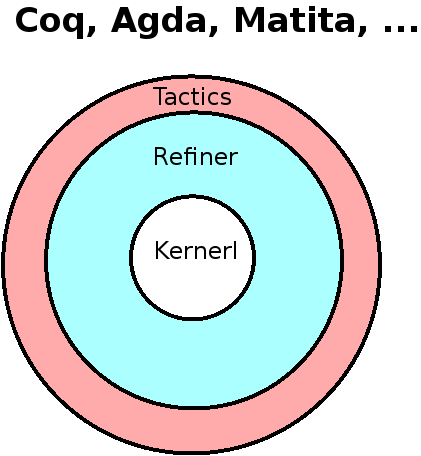
\includegraphics[width=0.9\textwidth]{architettura.png}
 \column{0.6\textwidth}
 \begin{block}{The Kernel}
  \begin{itemize}
   \item Works on \alert{ground terms/proofs}
   \item Syntax directed judgements + heuristics to speed up
    \begin{itemize}
     \item $\Gamma \vdash t : T$
     \item $\Gamma \vdash t_1 \equiv t_2$
     \item $\Gamma \vdash t \rhd t'$
    \end{itemize}
   \item Reduction/conversion via \alert{reduction machines}
   \item Needs to be FAST
  \end{itemize}
 \end{block}
\end{columns}
\end{frame}

\begin{frame}[fragile]
\frametitle{\small A Modular Implementation of a Type Checker for Proof Theory}
\begin{block}{Example: a reduction machine in $\lambda$Prolog/ELPI}
{\small
\begin{columns}[c]
 \column{0.3\textwidth}
$(\mathcal{E}, MN, \mathcal{S}) \longrightarrow$\\
$~~~(\mathcal{E}, M, [N|\mathcal{S}])$\\
~\\
$(\mathcal{E}, \lambda x.F, [N|\mathcal{S}]) \longrightarrow$\\
$~~~(\mathcal{E}\alert{[x \mapsto N]}, F, \mathcal{S})$
 \column{0.6\textwidth}
\begin{semiverbatim}
whd1 (app M N) S K :-
  K [] M [N|S].

whd1 (lam T F) [N|NS] K :-
  pi x \\ \alert{val x T N \textcolor{blue}{_NF}} =>
    K [x] (F x) NS.
\end{semiverbatim}
\end{columns}}
\end{block}

\begin{block}{Observations}
 \begin{enumerate}
  \item ``$\Rightarrow$'' is logically scoped: \alert{continuations} ``\texttt{K}'' required \alert{(CPS style)}; ``\texttt{[x]}'' to read-back the machine state at the end
  \item Teyjus is too restrictive about CPS: use ELPI
  \item \alert{Call-by-need:} \texttt{\textcolor{blue}{\_NF}} will be instantiated on-demand with the normal form of \texttt{N}
 \end{enumerate}
\end{block}
\end{frame}

\begin{frame}[fragile]
\frametitle{Evaluation}
 \begin{block}{Achievements}
  A \alert{kernel} that is \alert{almost equivalent} to the one of Matita 0.9
  but way more readable.
 \end{block}

 \begin{block}{Comparison with OCaml code}
  \begin{itemize}
  \item[+] \alert{no} logic-independent \alert{clutter} (De Bruijn indexes, lifting, etc.)
  \item[+] \alert{simple code}, very close to pen\&paper judgements\\
    (a kernel for Martin-L\"of TT by a student of math)
  \item[+] \alert{modular}:
   \begin{itemize}
     \item[+] add new rules later to extend the language
     \item[=] accumulate alternative implementations
   \end{itemize}
  \item[-] \alert{slow:} from 8x to 15x slower (\alert{ELPI vs interpreted OCaml})\\
   (Teyjus is even slower)
  \end{itemize}
 \end{block}
\end{frame}

\section{HOCLP}

\subsection{The need for HOCLP}

\begin{frame}[fragile]
\frametitle{\small Anatomy of an Interactive Theorem Prover for Type Theory}
\begin{columns}
 \column{0.4\textwidth}
 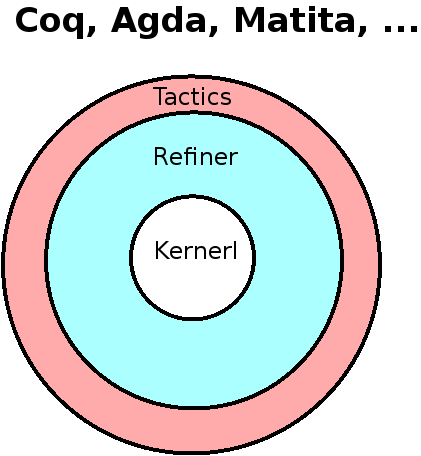
\includegraphics[width=0.9\textwidth]{architettura.png}
 \column{0.6\textwidth}
 \begin{block}{The Elaborator (Refiner)}
  \begin{itemize}
   \item Works on \alert{non-ground terms/proofs}
   \item On ground terms: should (\ldots) behave as the kernel
   \item Tons of \alert{heuristics}, \alert{fragile}, \alert{ever changing}, \alert{obscure code}
    \begin{itemize}
     \item $\Sigma: \Gamma \vdash t : T \leadsto \Sigma': t' : T'$
     \item $\Sigma: \Gamma \vdash t_1 \approx t_2 \leadsto \Sigma'$
    \end{itemize}
   \item Deterministic solutions to higher order unification problems
   \item Needs to be INTELLIGENT
   \item user-provided heuristics in LP style
  \end{itemize}
 \end{block}
\end{columns}
\end{frame}

\begin{frame}[fragile]
\frametitle{Representing open terms}
 \begin{block}{Open proofs/terms as non-ground terms}
  $$\frac{\uncover<2->{\alert{x:}}A, \uncover<2->{\alert{f:}}A \to B \vdash \uncover<2->{\alert{P\, x\, f} :} A}{\vdash \uncover<2->{\alert{\lambda x:A. \lambda f:A \to B. P\, x\, f :}} A \to (A \to B) \to B}$$
  \pause
 \end{block}

 \pause

 \begin{block}{Proof progress = metavariable instantiation}
  $$\alert{P\, x\, f} := \cblue{f~(Q\,x)}$$
  $$\frac{\dfrac{
     \dfrac{}{\alert{x:}A, \alert{f:}A \to B \vdash \alert{f :} A \to B} \quad \quad \begin{array}{c}~\\\alert{x:}A, \alert{f:}A \to B \vdash \alert{Q\,x:}A\end{array}
    }
    {\uncover<2->{\alert{x:}}A, \uncover<2->{\alert{f:}}A \to B \vdash \uncover<2->{\cblue{f~(Q\,x)} :} A}}
    {\vdash \uncover<2->{\alert{\lambda x:A. \lambda f:A \to B. \cblue{f~(Q\,x)} :}} A \to (A \to B) \to B}$$
 \end{block}

 \begin{block}{Type checking = partial correctness}
  The proof is correct \alert{so far}
 \end{block}
\end{frame}

\begin{frame}[fragile]
 \frametitle{The Hello-World of HOLP ($\lambda$Prolog)}
 \begin{block}{Type-Checking/Inference in $\lambda$Prolog}
  {\small
  \begin{semiverbatim}
of (app M N) B :- of M (arr A B), of N A.
of (lam F) (arr A B) :-
  pi x\\ of x A => of (F x) B.
  \end{semiverbatim}}
 \end{block}

 \begin{block}{Divergence on non-ground terms}
{\small
 \begin{semiverbatim}
   \{ \vvdash of (lam x \\ app \cblue{W} x) A \}
\alert{A \lleftarrow (arr B C)}
\mmapsto \{ of x B \vvdash of (app \cblue{W} x) C \}
\mmapsto \{ of x B \vvdash \cblue{of W (arr D C)}, of x B \vvdash of x D \}
\alert{W \lleftarrow (app W1 W2), \ldots}
\mmapsto \{ of x B \vvdash \cblue{of W1 (arr E (arr D C))},
  of x B \vvdash \cblue{of W2 E}, of x B \vvdash of x D \}
\alert{W1 \lleftarrow (app W11 W12), \ldots}
\ldots
 \end{semiverbatim}}
 \end{block}
\end{frame}

\begin{frame}[fragile]
 \frametitle{The Hello-World of HOCLP (ELPI)}
 \begin{block}{Expected behaviour in HOCLP}
  A \alert{recursive predicate} on a \alert{flexible term} is turned into a
  \cblue{constraint} added to a \cblue{constraint store}.
 \end{block}

 \begin{block}{Example behaviour on non-ground terms}
{\small
 \begin{semiverbatim}
   \{ \vvdash of (lam x \\ app W x) A \}, \cblue{\eemptyset}
\alert{A \lleftarrow (arr B C)}
\mmapsto \{ of x B \vvdash of (app W x) C \}, \cblue{\eemptyset}
\mmapsto \{ of x B \vvdash \alert{of W (arr D C)}, of x B \vvdash of x D \}, \cblue{\eemptyset}
\mmapsto \{ of x B \vvdash of x D \}, \cblue{\{ of x B \vvdash of W (arr D C) \}}
\alert{D \lleftarrow B}
\mmapsto \eemptyset, \cblue{\{ of x B \vvdash of W (arr B C) \}}
 \end{semiverbatim}}
 \end{block}

\uncover<2>{\begin{block}{Non-pattern-unification problems}
 Teyjus/ELPI: flex/flex case also delayed\\
 E.g. \cblue{$X~(f~x) = Y~x$}
\end{block}}
\end{frame}

\subsection{HOCLP: a proposal}

\begin{frame}[fragile]
 \frametitle{High-Level Syntax and Semantics}
\begin{block}{Syntax (example)}
\begin{semiverbatim}
\alert{delay (of X T) on X.}
of (app M N) B :- of M (arr A B), of N A.
of (lam F) (arr A B) :-
  pi x\\ of x A => of (F x) B.
\end{semiverbatim}
\end{block}

\begin{block}{Semantics of \texttt{delay}}
If $X$ is flexible (e.g. $Y~t_1~\ldots~t_n$), succeeds adding it to the constraint store.

~\\

\alert{Resume} the constraint when a query $Q$ instantiates $X$ to a rigid term In case of failure, \alert{backtrack} on $Q$.
\end{block}
\end{frame}

\begin{frame}[fragile]
\frametitle{Representing open terms}
 \begin{block}{Open proofs/terms as non-ground terms}
  $$\frac{\cblue{x:A, f:A \to B \vdash P\, x\, f : A}}{\vdash \lambda x:A. \lambda f:A \to B. P\, x\, f : A \to (A \to B) \to B}$$
 \end{block}

 \pause

 \begin{block}{Proof progress = metavariable instantiation}
  $$\cblue{P\, x\, f} := f~(Q\,x)$$
  $$\dfrac{
     \dfrac{}{x:A, f: A \to B \vdash f : A \to B} \quad \quad \begin{array}{c}~\\\cblue{x:A, f:A \to B \vdash Q\,x:A}\end{array}
    }
    {x:A, f:A \to B \vdash f~(Q\,x) : A}
    $$
 \end{block}
\end{frame}

\begin{frame}[fragile]
\frametitle{Accumulation of constraints}
 \begin{block}{One metavariable, two typing constraints}
 $$\frac{
   \cblue{f: \mathbb{N} \to \mathbb{B} \to \mathbb{N} \vdash X : \mathbb{N} \quad \quad f: \mathbb{N} \to \mathbb{B} \to \mathbb{N} \vdash X : \mathbb{B}}
   }{
   f: \mathbb{N} \to \mathbb{B} \to \mathbb{N} \vdash f~X~X : \mathbb{N}
   }$$

 \begin{itemize}
  \item When $X$ becomes ground, the constraint is checked \alert{twice}.
  \item The two constraints together are \alert{unsatisfiable}
 \end{itemize}
 \end{block}

 \begin{block}{Constraint Programming}
  \begin{itemize}
   \item Declare constraints
   \item Propagate constraints
    \begin{itemize}
     \item to detect early inconsistency
     \item to do \alert{forward reasoning} (beyond uniform proofs!)
    \end{itemize}
  \end{itemize}
 \end{block}
\end{frame}

\begin{frame}[fragile]
 \frametitle{CHR-style HOCLP}

\begin{block}{Constraint Handling Rules (CHR)-style propagation rules:}
{\small \begin{semiverbatim}
\textbf{constraint} list_of_constraint_heads \{
  S1 \textbf{\\} S2 \textbf{>} A \textbf{|} G \textbf{<=>} S3.
\}
\end{semiverbatim}}
\end{block}

\begin{block}{Example: unicity of typing}
{\small \begin{semiverbatim}
\textbf{constraint} of \{
  \textbf{rule} (G1 \textbf{?-} of X T1) \textbf{\\} (G2 \textbf{?-} of Y T2) \textbf{>} X \textbf{~} Y
       \textbf{|} (equiv G1 G2) \textbf{<=>} (\textbf{?-} T1 = T2).
\}
\end{semiverbatim}}
\end{block}

 \begin{block}{Operational semantics}
  \begin{enumerate}
   \item match (via $\sigma$) $S_1,S_2$ against the \alert{sintactic representation} of constraints in the store $S$ (up to the alignment mode $A$)
   \item execute the guard $G \sigma$ in a \alert{meta-interpreter}
   \item $S := S \setminus S_2 \sigma \cup S_3 \sigma$
  \end{enumerate}
 \end{block}
\end{frame}

\begin{frame}[fragile]
 \frametitle{CHR-style HOCLP}
 \begin{block}{What propagation rules can do}
  Rules compute in a meta-intepreter on the syntax of the logic below
  \begin{itemize}
   \item \alert{Meta-context} \texttt{Gamma} is a list of formulae
   \item \alert{Meta-meta-variables} are unified as usual
   \item \alert{Meta-variables are frozen} (can only be matched via \texttt{??}, \texttt{(?? as X)}, \texttt{(?X L)})
   \item \texttt{??} and \texttt{?? as X} match flexible terms
   \item \texttt{(?X L)} also \alert{decomposes} the flexible term into its head \texttt{X} and the list \texttt{L} of its arguments
   \item Instantiation of meta-variables can only be triggered when back in
    the interpreter
  \end{itemize}
 \end{block}
\end{frame}

\begin{frame}[fragile]
 \frametitle{Names and Alignments}
\begin{block}{CHR-like syntax (example)}
{\small \begin{semiverbatim}
\textbf{constraint} of \{
  \textbf{rule} (G1 \textbf{?-} of X T1) \textbf{\\} (G2 \textbf{?-} of Y T2) \textbf{>} X \textbf{~} Y
       \textbf{|} (equiv G1 G2) \textbf{<=>} (G1 \textbf{=>} T1 = T2).
\}
\end{semiverbatim}}
\end{block}

\begin{block}{Alignments}
 \begin{itemize}
  \item The \alert{free variables} of \texttt{G1 \textbf{?-} of X T1} are
    \alert{disjoint} from those of \texttt{G2 \textbf{?-} of X T2} and need
    to be \alert{aligned} using \alert{``equivariant matching''}
  \item Example:\\
   {\small \texttt{\{ (of x $\mathbb{Z}$ \textbf{?-} of (X x) $\mathbb{Z}$),\\~ (of y $\mathbb{Z}$ \textbf{?-} of (X y) $\mathbb{Z}$) \}}}
  \item \alert{Equivariant matching:} NP-complete
  \item Solution:
   \begin{enumerate}
    \item \alert{manual matching} in the guard
    \item pre-defined \alert{alignments}: \texttt{X x \textbf{\~} X y} matches
      \texttt{x} with \texttt{y}
   \end{enumerate}
    
 \end{itemize}
\end{block}
\end{frame}

\begin{frame}[fragile]
 \frametitle{Towards Certified HOCLP}
 \begin{block}{Constraint Handling Rules (CHR)-style propagation rules}
   A CHR-style rule is \alert{sound}
   and \alert{complete} w.r.t. the \alert{semantics on ground terms} iff
   $$S_1 \wedge G \Rightarrow (S_2 \Leftrightarrow S_3)$$
 \end{block}
 \begin{block}{CHR-style rule soundness}
  Every CHR-style rule should be proved sound and correct, i.e. we need to
  prove that a \alert{meta-theorem} holds \alert{on \cblue{small steps~(\ldots)}$\lambda$Prolog executions}.
 \end{block}

 \begin{block}{Abella: an Interactive Theorem Prover for $\lambda$Prolog}
\begin{thebibliography}{1}
\bibitem{Abella}
Andrew Gacek, Dale Miller, Gopalan Nadathur
\newblock {A two-level logic approach to reasoning about computations}.
\newblock{In {\em Journal of Automated Reasoning}, 49:241--273, 2012}.
\end{thebibliography}
 \end{block}
\end{frame}

\begin{frame}[fragile]
 \frametitle{Towards Certified HOCLP}
 \begin{block}{Is Abella the right tool?}
   \begin{tabular}{lll}Constraint propagation rules&=&meta-level computation\\
        Abella&=&meta-level reasoning\end{tabular}
  \begin{itemize}
   \item meta-meta-meta-\ldots level computations are possible\\
         but Abella's reasoning logic $\not =$ Abella's object logic
   \item meta-level computations on intermediate execution states\\
         but those are invisible to Abella's big step semantics
  \end{itemize}

  ~\\\alert{Future work: a small-step Abella}
 \end{block}
\end{frame}

\begin{frame}[fragile]
 \frametitle{Immediate Syntax}
{\small
 \begin{block}{Frequent case (especially for heuristics)}
  A query $Q$ is delayed to be immediately propagated by unary rules of the
  form \alert{$\emptyset \setminus Q~|~ G \Leftrightarrow Q'$}

  ~\\Costly: delay, quote, match, start meta-runtime, execute $G$, unquote $Q'$, stop meta-runtime
 \end{block}

 \begin{block}{Immediate syntax}
  \alert{Immediate syntax} to apply the rule \alert{before} delaying the goal.
  \begin{itemize}
   \item Example: \texttt{\textbf{mode} (of i o)}.
   \item Semantics: use \alert{matching (i)} on the first argument of \texttt{of}
   \item Match and propagate flexible terms via \texttt{??}, \texttt{(?? as X)}, \ldots
   \item Delay flexible terms explicitely if not propagated
  \end{itemize}

  ~\\ \alert{Semantically, it can be translated to CHR-style rules.}
 \end{block}}
\end{frame}

\begin{frame}[fragile]
 \frametitle{Immediate Syntax}
 \begin{block}{Immediate syntax example: narrowing}
{\small \begin{semiverbatim}
\alert{mode (comp i i i i i).}

% Case (T1 a1 \ldots) \aapprox m2
% Solution: T1 :- \llambda x. F
% \bbeta-step triggered before recursion
\alert{comp (?? as T1) [A|AS] M T2 L2 :-
 of A TYA,
 T1 = lam TYA F,
 pi x \ val x TYA A _NF => comp (F x) AS M T2 L2.}

% Heuristic: try PROJECTION first
% Case V1 \aapprox m2
% V1 := n-th argument X of the application
\alert{comp (?? as V1) [] M T2 S2 :-
 val X _ _ _,
 X = V1,
 comp V1 [] M T2 S2, !.}
\end{semiverbatim}}
 \end{block}
\end{frame}

\section{Conclusions}

\subsection{Conclusions and Future Work}

\begin{frame}[fragile]
 \frametitle{Higher Order Constraint Logic Programming (HOCLP)}

 \begin{block}{HOCLP (1st characterization)}
  HOCLP = HOLP + Constraint Handling Rules (CHR)

  \alert{Or how to exploit forward reasoning to reduce the search space}
 \end{block}

 \begin{block}{HOCLP (2nd characterization)}
  Minimal extension of HOLP to handle \alert{non-ground terms}.
 \end{block}
\end{frame}

\begin{frame}[fragile]
 \frametitle{Application Domains}
 \begin{columns}[t]
  \column{0.5\textwidth}
  \begin{block}{Ground terms with binders}
   \begin{itemize}
    \item formulae
    \item programming language syntax
    \item dependent types
   \end{itemize}
  \end{block}
  \begin{block}{HOLP}
   \begin{itemize}
    \item interpreters, compilers
    \item \alert{type and certificate/proof checkers}
    \item animated operational semantics
    \item hypothetical reasoning
   \end{itemize}
  \end{block}

  \column{0.5\textwidth}
  \begin{block}{Non-ground terms with binders}
   \begin{itemize}
    \item partial terms (user input)
    \item partial (dependent) types
    \item \alert{partial proofs}
   \end{itemize}
  \end{block}
  ~
  \begin{block}{HOCLP}
   \begin{itemize}
    \item type inference algorithm
    \item \alert{interactive theorem provers}
    \item ???
   \end{itemize}

   ~
  \end{block}
 \end{columns}
\end{frame}

\begin{frame}[fragile]
 \frametitle{Higher Order Constraint Logic Programming (HOCLP)}
 \begin{block}{HOCLP (3rd characterization)}
 \alert{The best} high-level language \alert{to implement interactive theorem provers}
 for dependently typed languages (Type Theory).
 \end{block}

 \begin{block}{Recipe for a certified modular elaborator (work in progress)}
  \begin{enumerate}
   \item declare \textbf{delay/mode}s for recursive predicates
   \item accumulate the kernel (\alert{FULL REUSE, NO CODE DUPLICATION}!)
   \item add (immediate or not) propagation rules
   \item prove all propagation rules to be sound (and some complete too)
   \item let the user tamper the heuristics with his own additional rules
   \item run some static analysis on the user augmented code
  \end{enumerate}
 \end{block}
\end{frame}

\subsection{Job Advertisement}

\begin{frame}
\frametitle{Advertisement}
\begin{block}{Open Post-Doc Position in Bologna}
Looking for a 1 year Post-Doc on one of the following topics
 \begin{itemize}
  \item implementation and optimization of HOCLP
  \item semantics of HOCLP
  \item static analysis of HOCLP code
  \item formal verification of HOCLP propagation rules
  \item implementation of type theory in HOCLP
 \end{itemize}

~\\\alert{Contact: \texttt{claudio.sacerdoticoen@unibo.it}}
\end{block}
\end{frame}

\end{document}

\section{ELPI: an HOCLP Implementation}

\subsection{High Level Commands}

\begin{frame}[fragile]
 \frametitle{High-Level Syntax and Semantics}
\begin{block}{Syntax (example)}
\begin{semiverbatim}
\alert{delay (of X T) on X.}
of (app M N) B :- of M (arr A B), of N A.
of (lam A F) (arr A B) :-
  pi x\\ of x A => of (F x) B.
\end{semiverbatim}
\end{block}

\begin{block}{Semantics}
A query \texttt{(of (X $t_1$ \ldots $t_n$) T)} is \alert{delayed} and put in the
\alert{constraint store}. Computation continues with the next query in the stack.


When a query $Q$ instantiates \texttt{(X $t_1$ \ldots $t_n$)} to a rigid term $\mathcal{T}$, \texttt{(of $\mathcal{T}$ T)} is \alert{resumed}. If it fails, it triggers \alert{backtracking} on $Q$.
\end{block}
\end{frame}

\begin{frame}[fragile]
 \frametitle{High-Level Syntax and Semantics}
\begin{block}{CHR-like syntax (example)}
{\small \begin{semiverbatim}
\textbf{constraint} of \{
  \textbf{rule} (G1 \textbf{?-} of X T1) \textbf{\\} (G2 \textbf{?-} of Y T2) \textbf{>} X \textbf{~} Y
       \textbf{|} (equiv G1 G2) \textbf{<=>} (G1 \textbf{=>} T1 = T2).
\}
\end{semiverbatim}}
\end{block}

\begin{block}{Semantics}
When a constraint of type ``\texttt{of}'' enters the constraint store, it immediately triggers \alert{propagation} according to the rules in the \texttt{\textbf{constraint}} block. The order of application of propagation rules is determined by the \alert{standard CHR semantics}.
\end{block}
\end{frame}
 
\begin{frame}[fragile]
 \frametitle{High-Level Syntax and Semantics}
\begin{block}{CHR-like syntax (example)}
{\small \begin{semiverbatim}
\textbf{constraint} of \{
  \textbf{rule} (G1 \textbf{?-} of X T1) \textbf{\\} (G2 \textbf{?-} of Y T2) \textbf{>} X \textbf{~} Y
       \textbf{|} (equiv G1 G2) \textbf{<=>} (G1 \textbf{=>} T1 = T2).
\}
\end{semiverbatim}}
\end{block}

\begin{block}{Meta-Level computation}
Propagation rules inspect the \alert{syntax} of delayed goals:
\begin{itemize}
 \item \texttt{G1, G2} are list of predicates (contexts)
 \item \texttt{X,Y} match the syntax of flexible terms
 \item the arguments $t_1,\ldots,t_n$ of \texttt{X,Y} can be inspected
   as lists
 \item rules applied up to \alert{matching} only (no unification)
 \item \texttt{X \textbf{\~} Y} is an \alert{alignment}: (see later)
\end{itemize}
\end{block}
\end{frame}

\begin{frame}[fragile]
 \frametitle{Meta-Level Computations}
\begin{block}{CHR-like syntax (example)}
{\small \begin{semiverbatim}
\textbf{constraint} of \{
  \textbf{rule} (G1 \textbf{?-} of X T1) \textbf{\\} (G2 \textbf{?-} of Y T2) \textbf{>} X \textbf{~} Y
       \textbf{|} (equiv G1 G2) \textbf{<=>} (G1 \textbf{=>} T1 = T2).
\}
\end{semiverbatim}}
\end{block}

 \begin{block}{Implementation}
  \begin{itemize}
   \item \texttt{(equiv G1 G2)} is executed in a \alert{meta-level run-time}
     that works on the \alert{syntax of the run-time}
   \item meta-meta-\ldots-level run-times are possible
   \item cfr: meta-level run-time $\approx$ meta-level logic of Abella
   \item new goal \texttt{G1 \textbf{=>} T1 = T2} returned to the run-time
     and executed in the empty context (i.e. after one step $G1 \vdash T1 = T2$)
  \end{itemize}
 \end{block}
\end{frame}

\begin{frame}[fragile]
 \frametitle{Names and Alignments}
\begin{block}{CHR-like syntax (example)}
{\small \begin{semiverbatim}
\textbf{constraint} of \{
  \textbf{rule} (G1 \textbf{?-} of X T1) \textbf{\\} (G2 \textbf{?-} of Y T2) \textbf{>} X \textbf{~} Y
       \textbf{|} (equiv G1 G2) \textbf{<=>} (G1 \textbf{=>} T1 = T2).
\}
\end{semiverbatim}}
\end{block}

\begin{block}{Alignments}
 \begin{itemize}
  \item The \alert{free variables} of \texttt{G1 \textbf{?-} of X T1} are
    \alert{disjoint} from those of \texttt{G2 \textbf{?-} of X T2}
  \item Example:\\
   {\small \texttt{\{ (of x $\mathbb{Z}$ \textbf{?-} of (X x) $\mathbb{Z}$),\\~ (of y $\mathbb{Z}$ \textbf{?-} of (X y) $\mathbb{Z}$) \}}}
  \item \alert{Equivariant matching:} NP-complete
  \item Solution:
   \begin{enumerate}
    \item \alert{manual matching} in the guard
    \item pre-defined \alert{alignments}: \texttt{X x \textbf{\~} X y} matches
      \texttt{x} with \texttt{y}
   \end{enumerate}
    
 \end{itemize}
\end{block}
\end{frame}

\begin{frame}[fragile]
 \frametitle{Immediate Syntax}
 \begin{block}{Frequent case}
  A query $Q$ is delayed to be immediately propagated by unary rules of the
  form \alert{$\emptyset \setminus Q~|~ G \Leftrightarrow Q'$}

  ~\\Costly: delay, quote, match, start meta-runtime, execute $G$, unquote $Q'$, stop meta-runtime
 \end{block}

 \begin{block}{Immediate syntax}
  \alert{Immediate syntax} to apply the rule \alert{before} delaying the goal.
 \end{block}
\end{frame}

\begin{frame}[fragile]
 \frametitle{Immediate Syntax}
 \begin{block}{Immediate Syntax: example}
\begin{semiverbatim}
\textbf{mode} (leq \textbf{i} \textbf{i}).
leq 0 0.
leq X Y :- leq X Z, Y \textbf{is} X + 1.
leq (?? as X) (?? as X).
leq (?? as X) (?? as Y) :- $delay (leq X Y) (X;Y).
\end{semiverbatim}
 \end{block}

 \begin{block}{Semantics}
 \end{block}
\end{frame}

\section{Implementing Type Theory in HOCLP}


\begin{frame}[fragile]
 \frametitle{Higher Order Logic Programming for\\ Type/Proof Checking}

 Curry-Howard: \alert{proof checking} is \alert{type checking}.\\~\\

 $$
  \frac{\Gamma \vdash M : A \to B \quad \Gamma \vdash N : A}{\Gamma \vdash M N : B}
  \quad \quad
  \frac{\Gamma, x: A \vdash M : B}{\Gamma \vdash \lambda x:A. M : A \to B}
 $$

\pause
 ~\\~\\HOLP ($\lambda$Proplog / LF / \ldots) great for\\\alert{binders} and \alert{derivation rules}:

\begin{verbatim}
of (app M N) B :- of M (arr A B), of N A.
of (lam F) (arr A B) :- pi x\ of x A => of (F x) B.
\end{verbatim}\\

\end{frame}

\begin{frame}[fragile]
 \frametitle{Curry-Howard for Partial Proofs}

 Curry-Howard: \alert{partial proof} is \alert{partial term}.\\

 $$\uncover<3->{t ::= \ldots ~|~ Y[t,\ldots,t] \quad \quad \mbox{explicitly substituted metavariable}}$$

 $$
  \frac{\uncover<2->{x:} A \vdash \uncover<2->{\only<2>{\alert{?}}\only<3->{\alert{Y[x]}}:} A}{\vdash \uncover<2->{\lambda x:A.} \only<2->{\only<2>{\alert{?}}\only<3->{\alert{Y[x]}}:} A \to A}
 \uncover<4->{{\Longleftarrow \mbox{when does it hold?} \atop ~}}
 $$

 \pause
 \pause
 \pause
 \pause

 ~\\

 $$
  \frac{(x:A \vdash Y[x] : B) \in \alert{\Sigma} \quad
         \alert{\Sigma;}\Gamma \vdash t : A}{\alert{\Sigma;}\Gamma \vdash X[t] : B}
 $$
 
 \pause

 {\small
 ~\\plus instantiation, reduction, management of explicit substitutions, \ldots \quad \quad \alert{Coq, Matita, Agda, Lean, \ldots}\\\pause
 plus metatheorems about instantiation, commutation with substitution, reduction, typing, \ldots
 }

\end{frame}

\begin{frame}[fragile]
 \frametitle{Failure of Higher Order Logic Programming for\\ Partial Proof Checking / Elaboration}

 Stop reinventing the wheel!\\~\\

 Shallow encoding in HOLP: $\alert{Y[x] = Y~x}$.\\~\\

 $$
  \frac{x: A \vdash \alert{Y~x}: A}{\vdash \lambda x:A.\alert{Y~x}: A \to A}
  \uncover<2->{{\Longleftarrow \mbox{when does it hold?} \atop ~}}
 $$

\uncover<3->{
HOLP semantics: blind term enumeration (\alert{WRONG!})\\~\\

\small{
\begin{tabular}{ll}
& \texttt{of (app X Y) Z}\\
$\Leftarrow$ & \texttt{of X (arr A Z), of Y A}\\
$\Leftarrow$ & \alert{\texttt{X = app X1 X2}}
               \texttt{, of X1 (arr B (arr A Z)), of Y A}\\
$\Leftarrow$ & \alert{\texttt{X1 = app X11 X12}}, \ldots\\
$\Leftarrow$ & \ldots
\end{tabular}}
}

\end{frame}

\begin{frame}[fragile]
 \frametitle{Higher Order Constraint Logic Programming for\\ Partial Proof Checking / Elaboration}

 Stop reinventing the wheel!\\~\\

 Shallow encoding in HOLP: $\alert{Y[x] = Y~x}$.\\~\\

 $$
  \frac{x: A \vdash \alert{Y~x}: A}{\vdash \lambda x:A.\alert{Y~x}: A \to A}
  {\Longleftarrow \mbox{\alert{this is a CONSTRAINT over $Y$!}} \atop ~}
 $$

 ~\\~\\HOCLP semantics:\\~

 \begin{enumerate}
  \item the goals is delayed over $Y$, i.e. it is turned into a \alert{constraint}
  \item if/when $Y$ is instantiated, the goal is \alert{resumed}
  \item works \alert{uniformly and for free on all judgments}: substituion, reduction, typing,
    strict positivity conditions, size (universe) constraints, \ldots
 \end{enumerate}

\end{frame}

\begin{frame}[fragile]
 \frametitle{Constraint Propagation}

 \alert{The semantics of a constraint is given for free from the semantics of its ground instances.}\\~\\

 \quad\alert{Constraint propagation}\\ $\equiv$ \alert{Forward reasoning} over constraints\\ $\subseteq$ meta-theorems of the logic\\~\\

 Example: \alert{Unicity of typing} propagation rule\\

 $$\begin{array}{l}(\Gamma \vdash X~\Gamma : T_1) \Rightarrow\\
   \quad \quad (\Gamma \vdash X~\Gamma : T_2) \iff (\Gamma \vdash T_1 = T_2)
   \end{array}$$

 ~\\Operationally: replace the second constraint with the third.\\\pause
 Requires constraint matching up to AC for $\Gamma$ and \alert{equivariance}.
\end{frame}

\begin{frame}[fragile]
 \frametitle{Work in Progress}
 \begin{itemize}
  \item ELPI: an \alert{interpreter} for $\lambda$Prolog + constraint propagation\\
   (\`a la CHR)
  \item Better understanding of the primitives required\\
    (in progress)
  \item A type-checker for Landau's Grundlagen in Automath (only 3x slower than interpreted OCaml code); an HOL theorem prover (very slow); a Matita implementation (in progress, 25x slower atm)
 \end{itemize}

 ~\\ Major \alert{trade-off} between expressivity and \alert{performance}\\(to be quantified).
\end{frame}

\begin{frame}[fragile]
 \frametitle{Conclusions}
 \begin{itemize}
  \item proof assistant code becomes much \alert{smaller}, more \alert{modular}
   and \alert{simpler} (no De Brujin indexes, $\Sigma$s, \ldots)
  \item \alert{logic independent} code (for binders, metavariables, unification, etc.) moved from Matita to the ELPI interpreter and optimized
  \item the \alert{core algorithms} (e.g. unification, elaboration) and its \alert{extensions in user space} (coercions, canonical structures, type classes) written in \alert{the same language} as additional rules
  \item Propagation rules can be \alert{certified} in Abella (almost\ldots)
 \end{itemize}
\end{frame}

\end{document}

\section{$\lambda$Prolog: syntax \& semantics}

\begin{frame}
 \frametitle{$\lambda$Prolog}
 $\lambda$Prolog is a superset of Prolog\\~\\

 handles \alert{higher-order abstract syntax}\\~\\

 Example: $\int_0^1 \sin x~dx$ $~=~$ \texttt{integral 0 1 x\bs sin x}\\~\\

 where:
 \begin{enumerate}
   \item \texttt{x\bs f x} is $\lambda$-abstraction (i.e. $\lambda x. f~x$)
   \item \texttt{integral} has type $\mathbb{R} \to \mathbb{R} \to (\mathbb{R} \to \mathbb{R}) \to \mathbb{R}$
 \end{enumerate}
\end{frame}

\begin{frame}
 \frametitle{$\lambda$Prolog}

 Does NOT mix functional and logic programming\\~\\

 $\beta$-reduction is not responsible for computation\\~\\

 $\beta$-reduction used for\\
 \begin{enumerate}
  \item renaming (bound) variables
  \item substitution
 \end{enumerate}
\end{frame}

%\begin{frame}
% \frametitle{$\lambda$Prolog}
% $\lambda$Prolog avoids most non-logical tricks:\\~\\
%
% \begin{tabular}{clc}
% $\lambda$Prolog &~~~~vs~~~~& Prolog \\~\\
% \texttt{for\_all (x\bs p x) L} && \texttt{for\_all (p X) X L}\\~\\
% logical implication \texttt{=>} && \texttt{assert/retract}
% \end{tabular}
%\end{frame}

\begin{frame}
 \frametitle{$\lambda$Prolog}

  Syntax:\\~\\

  \begin{tabular}{ll}
  \begin{tabular}{llll}
  \texttt{Q} & ::= & PRED & predicate\\
             & $|$ & \texttt{true} & true\\
             & $|$ & \texttt{sigma X\bs Q} & existential quantification\\
             & $|$ & \texttt{Q,Q} & conjunction\\
             & $|$ & \texttt{Q;Q} & disjunction\\
             & $|$ & \texttt{\alert{C => Q}} & \alert{implication}\\
             & $|$ & \texttt{\alert{pi x\bs Q}} & \alert{universal quantification}
  \end{tabular}
  & query\\

  \texttt{C ::= PRED | true | pi X\bs C | C,C | Q => C} & clause\\


  \texttt{\alert{PRED ::= TERM}} & predicate\\

  \texttt{TERM ::= x | X | TERM~TERM | \alert{x\bs TERM} | \alert{Q} } & term\\
 \end{tabular}
\end{frame}

\begin{frame}
 \frametitle{$\lambda$Prolog}
 Semantics:\\~\\

 \begin{tabular}{cl}
 $\frac
  {\Gamma, \mbox{\texttt{C}}~\vdash~\mbox{\texttt{Q}}}
  {\Gamma~\vdash~\mbox{\texttt{C=>Q}}}
 $
 &
 \begin{tabular}{l}
 The program $\Gamma$ is temporarily\\
 augmented with the clause \texttt{C}
 \end{tabular}
 \\~\\

 $\frac
  {\Gamma~\vdash~\mbox{\texttt{Q[y/x]}} \quad\mbox{$y$ fresh}}
  {\Gamma~\vdash~\mbox{\texttt{pi x\bs Q}}}
 $
 &
 \begin{tabular}{l}
 A fresh constant is temporarily\\
 introduced.
 \end{tabular}
 \\~\\

 \begin{tabular}{l}
 \texttt{PRED ::= TERM}\\
 \texttt{TERM ::= \ldots | Q}\\
 \texttt{eval X :- X}
 \end{tabular}
 &
 \begin{tabular}{l}Dynamic code evaluation.\end{tabular}
 \\~\\

 binders and $\beta$-redexes
 &
 $\alpha$-conversion and $\beta$-reduction
 \end{tabular}
\end{frame}


\begin{frame}
 \frametitle{$\lambda$Prolog}
 unification is \alert{higher order}\\(i.e. up to $\alpha$-conversion and $\beta$-reduction)\\~\\

 \alert{no most general unifier}\\~\\

 \begin{tabular}{lc}
 Example: & $F~a = a + a$\\
 Solutions: &
 $\begin{array}{l@{~~~}l}F_1 := \lambda x. a+a & F_2 := \lambda x. a+x\\ F_3 := \lambda x. x+a & F_4 := \lambda x.x+x\end{array}$
 \end{tabular}
\\~\\~\\
 
 unification is \alert{undecidable}
\end{frame}

\begin{frame}
 \frametitle{Pattern Fragment}
 $X~c_1~\ldots~c_n$ with all $c_i$ distinct and not in the scope of $X$\\~\\

 \alert{unique, most general unifier}\\~\\

 fragment \alert{stable} by computation\\~\\

 very expressive; most code naturally fits in the fragment\\~\\

 traversal of expressions fits in the fragment
\end{frame}

\begin{frame}
 \frametitle{$\lambda$Prolog}
 binders introduce \alert{local constants}\\~\\

 unification occurs under a \alert{mixed prefix}\\~\\

 Example: $\forall f\, \exists F\, \forall a~b\, \exists G, F~a = f~G$\\~\\
 Solution:
  $\begin{array}{l}
    F := \lambda a. f~G'\\
    G := G'\\
    \mbox{$b$ fresh for $G'$}
  \end{array}$
\end{frame}

\section{The two uses of $\beta$-reduction}

\begin{frame}[fragile]
 \frametitle{Simply typed $\lambda$-calculus in $\lambda$Prolog}
\texttt{app:}$\tau \to \tau \to \tau$
$\quad$
\texttt{lam:}$(\tau \to \tau) \to \tau$
$\quad$
\texttt{arr:}$\star \to \star \to \star$\\
Example: $\lambda x.x~x$ = \texttt{lam x\bs app x x}

~\\

Type checking/type inference: \texttt{of:} $\tau \to \star \to o$
\begin{verbatim}
of (app M N) B :- of M (arr A B), of N A.
of (lam F) (arr A B) :- pi x\bs of x A => of (F x) B.
\end{verbatim}\\

~\\

Call-by-name reduction: \texttt{cbn:} $\tau \to \tau \to o$
\begin{verbatim}
cbn (lam F) (lam F).
cbn (app M N) R :- cbn M (lam F), cbn (F N) R.
\end{verbatim}
\end{frame}

\begin{frame}
 \frametitle{First use of $\beta$-reduction}

 To traverse a binder \texttt{b F} (where \texttt{F = y\bs} $\mathcal{M}$)
  \begin{itemize}
   \item Pick a fresh name with \texttt{pi x\bs \ldots}
   \item Apply \texttt{F} to \texttt{x} to compute $\mathcal{M}$[x/y]
  \end{itemize}~\\

 \texttt{of (lam F) (arr A B) :-\\~~~ \alert{pi x\bs} of x A => of \alert{(F x)} B.}\\~\\

 \pause

 \uncover<2,3>{
 \begin{tabular}{ll}
 & \texttt{of \alert{(lam y\bs app f y)} Z}\\
 $\Leftarrow$ &
 \texttt{Z = arr A B,} \\ &
 \texttt{of x A $\vdash$ of \alert{((lam y\bs app f y) x)} B}\\
 = &
 \texttt{Z = arr A B,} \\ &
 \texttt{of \alert{x} A $\vdash$ of \alert{(app f x)} B}\\
 \end{tabular}
 \\~\\}

 \pause

 \alert{Morally not a reduction: only a way to name the bound variable.}\\~\\

 \pause

 \alert{Extremely frequent (structural recursion over syntax)}

 ~\\It fits the pattern fragment
\end{frame}

\begin{frame}
 \frametitle{Second use of $\beta$-reduction}

 To delegate instantiation/substitution at the meta-level\\~\\

 \texttt{\hspace{-0.25cm}
  cbn (app M N) R :- cbn M (lam F), cbn (\alert{F N}) R.
 }

 \alert{Performed rarely}

 ~\\It escapes the pattern fragment

 ~\\\alert{Avoidable with some effort in presence of delays}\\
 Hint: \begin{tabular}{l}implement a substitution predicate,\\ delay on existential variables\end{tabular}
\end{frame}

\begin{frame}
 \frametitle{$\beta$-reduction and backtracking}

 \uncover<1,2>{
 $\beta$-reduction triggers substitution\\~\\

 immediate propagation is costly (multiple traversals)\\~\\

 backtracking can make substitution steps useless\\~\\
 }

 \pause

 Teyjus: use explicit substitutions\\~\\

 \texttt{(x\ m n) t} $\rightarrow$ \texttt{(m n)[t/x]} $\rightarrow$ \texttt{m[t/x] n[t/x]} $\rightarrow$ \ldots

 \pause

 ~\\Not great idea
 \begin{itemize}
   \item too much pressure on \alert{garbage collection}
   \item fixed \alert{overhead} in every function\\
         (Prolog fragment slows down)
   \item most reductions are morally \alert{useless} anyway
 \end{itemize}
\end{frame}

\begin{frame}
 \frametitle{Avoiding $\beta$-reduction}

 Use \alert{hereditary substitutions}\\
 \begin{itemize}
   \item $\beta$-redexes are not part of the syntax
   \item when a substitution would create a $\beta$-redex,\\
         it triggers another substitution
 \end{itemize}

 $$(X~c)[\lambda x.t/X] \rightarrow t[c/x]$$

 ~\\reduced overhead to compute weak head normal forms
\end{frame}

\begin{frame}
 \frametitle{Avoiding $\beta$-reduction}

 Use \alert{De Brujin LEVELS}\\~\\

 if $n \geq 0$ then $n$ is the $(n+1)-th$ variable bound from outside\\
 if $n < 0$ then $n$ is a global constant\\~\\

 $$\lambda \alert{x}. f~\alert{x}~(\lambda y. g~\alert{x}~y)
 = \lambda. -1~\alert{0}~(\lambda. -2~\alert{0}~1)$$

 ~\\constants and variables handled uniformly

 ~\\the variable $x$ has the same number in every context
\end{frame}

\begin{frame}
 \frametitle{Avoiding $\beta$-reduction}

 The \alert{reduction-free fragment}:\\~\\

 all existential variables occur as $X^n_m$ where\\~\\

 $X^n_m$ stands for $X~n~\ldots~(n+m)$\\
 when all variables in $(-\infty,n)$ are in scope for $X$\\~\\

 \begin{itemize}
  \item is a sub-fragment of the pattern fragment
    \begin{itemize}
     \item decidability of unification
     \item unique and most general unifier
    \end{itemize}
  \item extremely frequent case
  \item admits constant time $\beta$-reduction and unification
  \item is not stable by computation
 \end{itemize}
\end{frame}

\begin{frame}
 \frametitle{Avoiding $\beta$-reduction}

 Constant time $\beta$-reduction:\\~\\

 assume $0 \ldots (n-1)\vdash X^n := \lambda. \ldots \lambda. t\quad$ Then\\

 \begin{center}
 $X^n_m = (\lambda. \ldots. \lambda. t)~n~\ldots~(n+m)
 = t[n/n]\ldots[n+m/n+m] = t$
 \end{center}

~\\

The first use of $\beta$-reduction is in the fragment:\\~\\

{\small
\texttt{
\hspace{-0.2cm}
of (lam F) (arr A B) :- pi x\bs of x A => of (F x) B.\\
\hspace{5cm}=\\
\hspace{-0.75cm}
\alert{$\forall n$.}(of (lam \alert{F$^n_0$}) (arr A B) :- pi x\bs of x A => of \alert{F$^n_1$} B).
}}
\end{frame}

\begin{frame}
 \frametitle{Avoiding $\beta$-reduction}

 \alert{Constant time unification}: $X^n_m = t$\\~\\

 Outside the fragment: $\beta$-reduction is implemented \alert{naively}\\~\\

 Most other operations can be \alert{optimized} for the $X^n_m$ representation\\~\\

 Tricky point: $X^n_m$ can be generated dinamically
\end{frame}

\section{Conclusions and future works}

\begin{frame}
 \frametitle{Conclusions}
 \begin{itemize}
  \item we have identified an unstable fragment of $\lambda$Prolog that
   covers most uses
  \item hereditary substitutions + De Brujin levels = reduction free handling
   of the fragment in most cases
  \item $>$ 50x speed up over Teyjus explicit substitution mechanism (in the fragment)
  \item $\approx$ 2x speed up over Teyjus with only 4\% of the code\\
    (carefully ingeneered implementation,\\
     1 year of optimizations,\\
     required some deep knowledge on OCaml internals)
 \end{itemize}
\end{frame}

\begin{frame}
 \frametitle{Future works}
 \begin{itemize}
  \item integration with CHR-style Constraint Programming
  \item re-implementation of the elaborator of Coq/Matita
  \item compilation (can we become 5x faster?)
 \end{itemize}
\end{frame}

\end{document}
